\documentclass[tikz,14pt,fleqn]{article}

% Math
\usepackage[fleqn]{amsmath}
\usepackage{amssymb}
\usepackage{dsfont}
\usepackage{float}

% Insert dummy text
\usepackage{lipsum}  
% Allows to use caption*
\usepackage{caption}
% Scalabale subfigures
\usepackage{subcaption} 
% Code syntax highlighting
\usepackage{minted}
% Hyperlinks
\usepackage{hyperref}
% Customize page layout
\usepackage{geometry}
\geometry{a4paper, margin=1in}
% Page headers and footers
\usepackage{fancyhdr}
\pagestyle{fancy}
\fancyhf{}
\setlength{\parindent}{0pt}
\setlength{\parskip}{0.5\baselineskip}%

% includegraphics
\usepackage{graphicx}




\newcommand{\bmat}[1]{
   \ensuremath{
   \begin{bmatrix}
       #1
   \end{bmatrix}
}}




\usepackage[utf8]{inputenc}


%%%%%%%%%%%%%%%%%%%%%%%%%%%%
%% VARIABLES
\newcommand\namesurname{Albert Cerfeda}
\newcommand\assignment{Assignment 1}

\newcommand\subject{Image \& Video Processing}
\newcommand\documentdate{19 March 2023}

% Title content
%%%%%%%%%%%%%%%%%%%%%%%%%%%%
\rhead{\assignment}
\lhead{\namesurname}
%%%%%%%%%%%%%%%%%%%%%%%%%%%%

\rfoot{Page \thepage}


\begin{document}

\begin{titlepage}
   \begin{center}
       \vspace*{0.2cm}

       \textbf{\Large{\subject}}

       \vspace{0.5cm}
        \textbf{\assignment}\\[5mm]
        
            
       \vspace{0.4cm}

        \namesurname
        \begin{figure}[H]
            \centering
        \end{figure}
       \tableofcontents

       \vspace*{\fill}
     
        
\includegraphics[width=0.4\textwidth]{fig/logo.png}
       
        \documentdate \\
        Università della Svizzera italiana\\
        Faculty of Informatics\\
        Switzerland\\

   \end{center}
\end{titlepage}

\section{Point Operations [20 points]}


\subsection{Tone mapping \& Linearization [2 points]}

\begin{figure}[h!]
    \begin{subfigure}{0.5\textwidth}
        \centering
        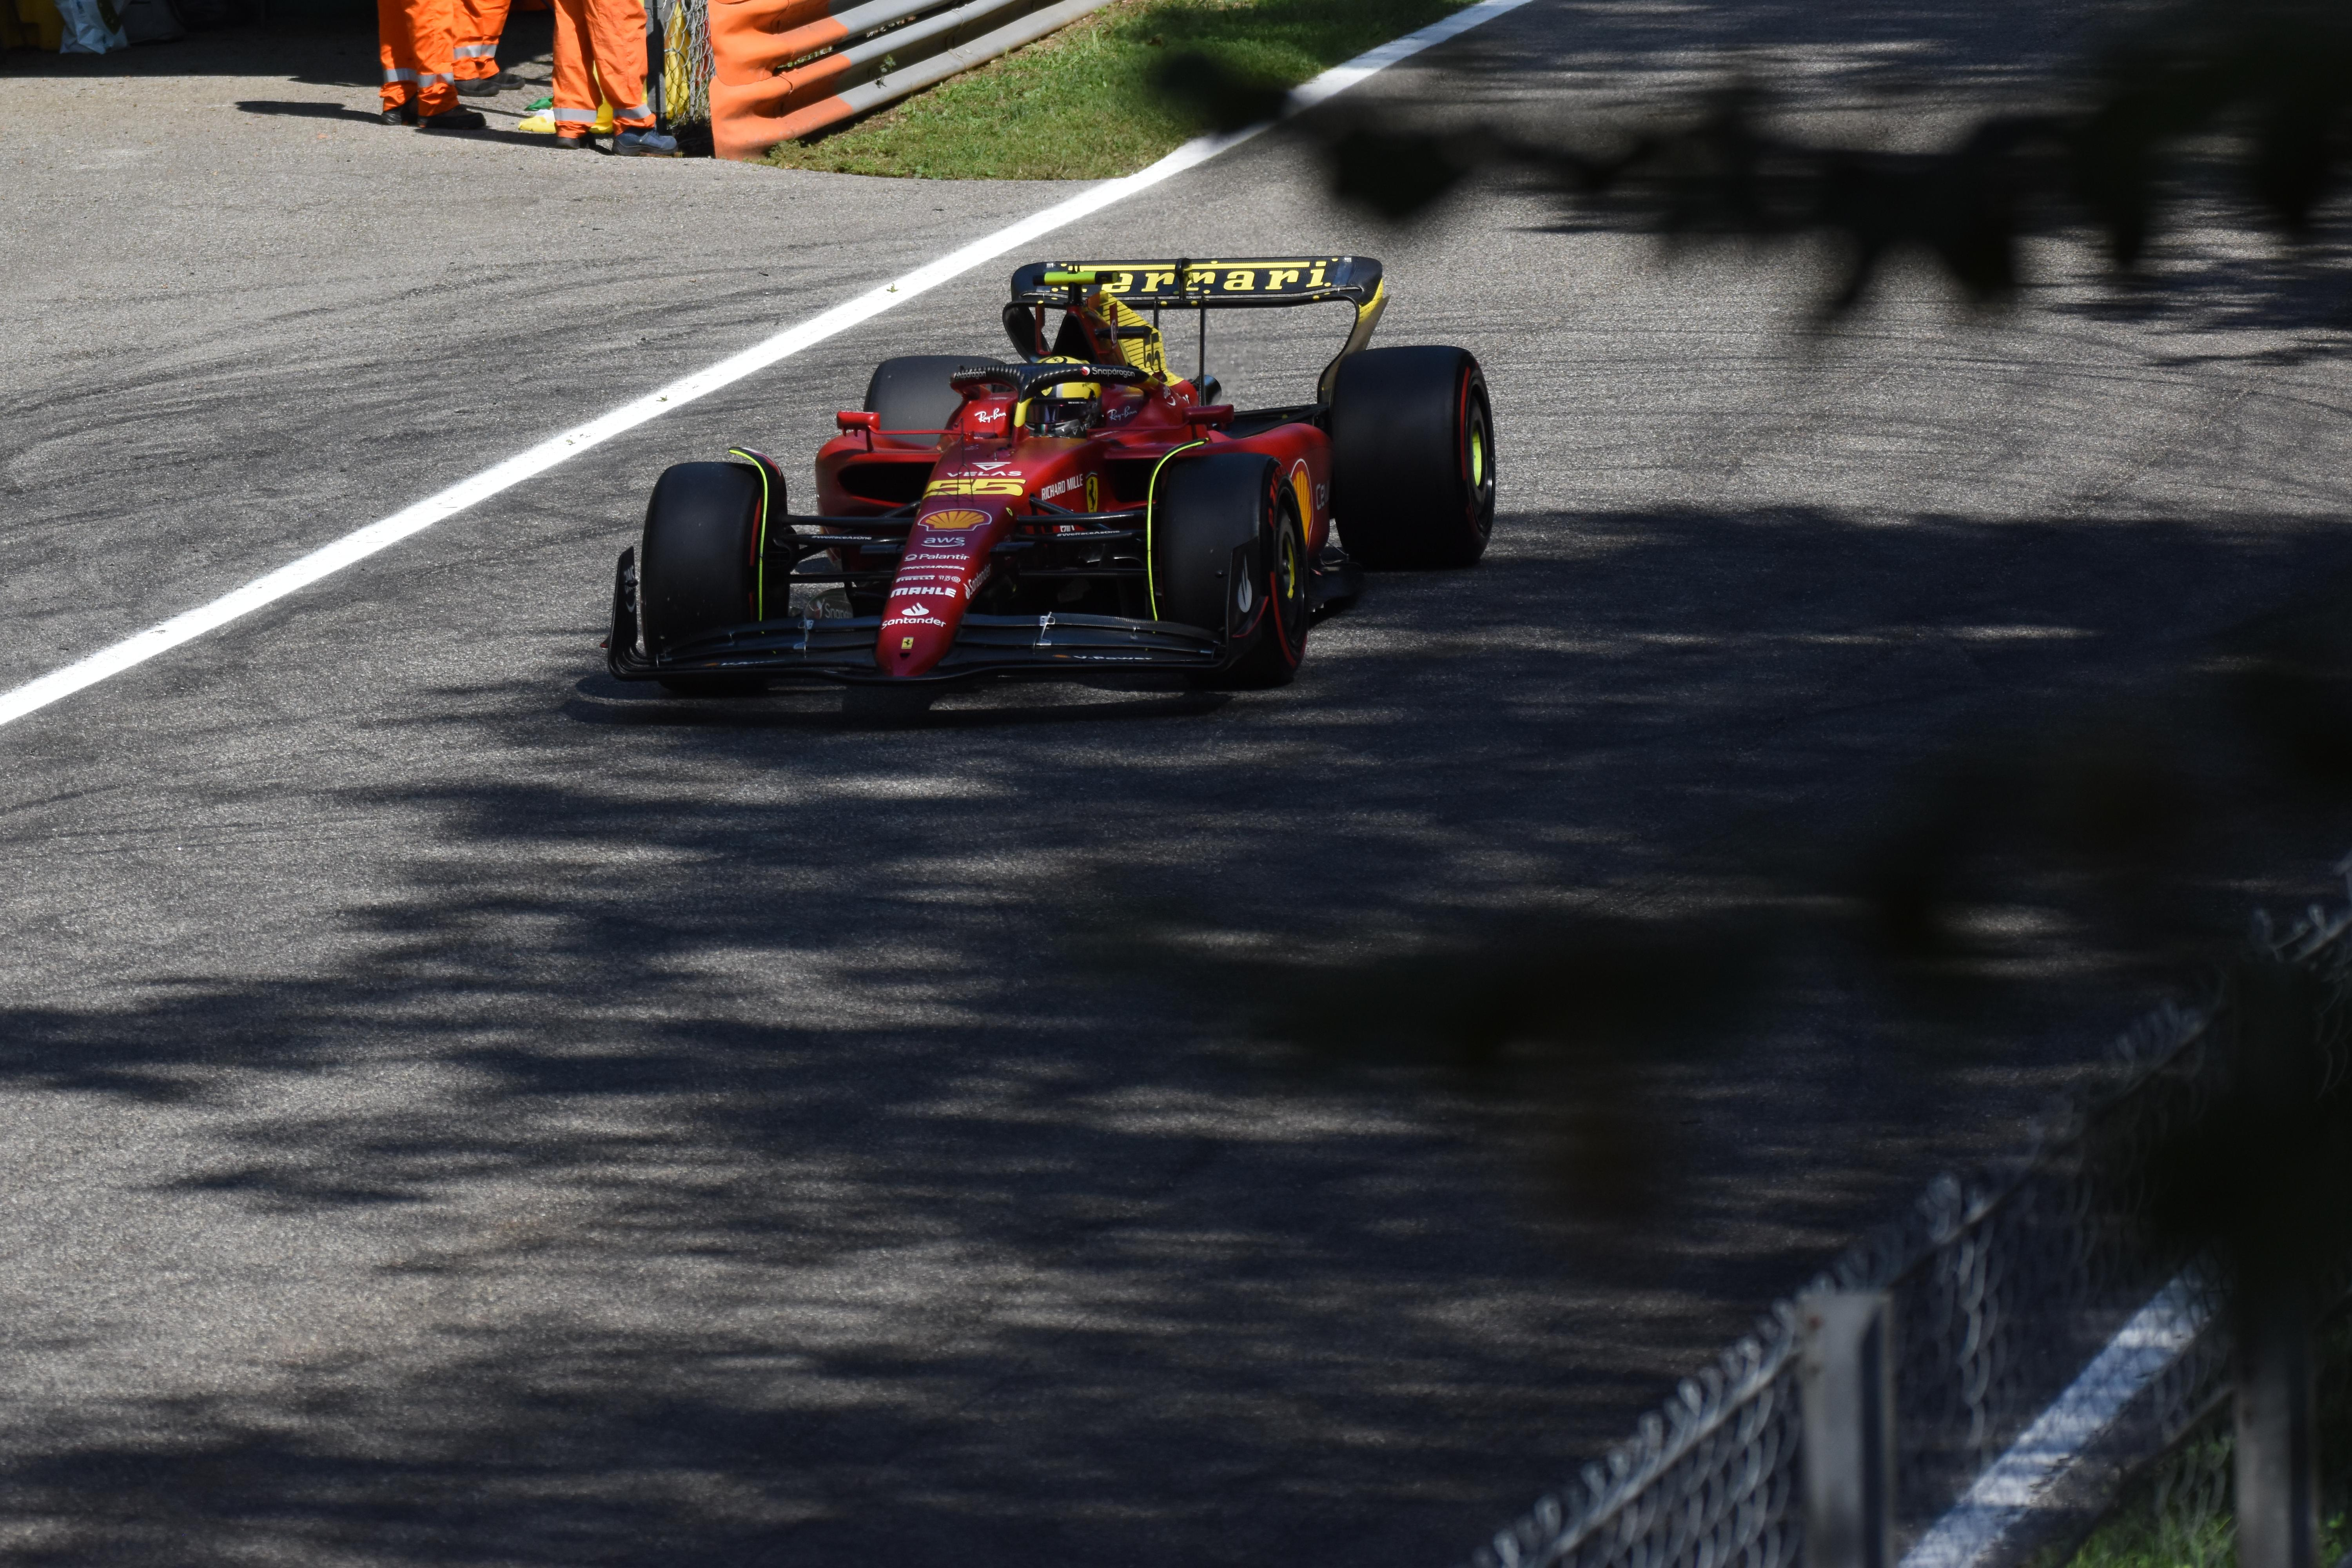
\includegraphics[width=\textwidth]{fig/out/1.ferrari.jpg}
        \caption{Original $\texttt{ferrari.jpg}$.}
    \end{subfigure}
    \begin{subfigure}{0.5\textwidth}
        \centering
        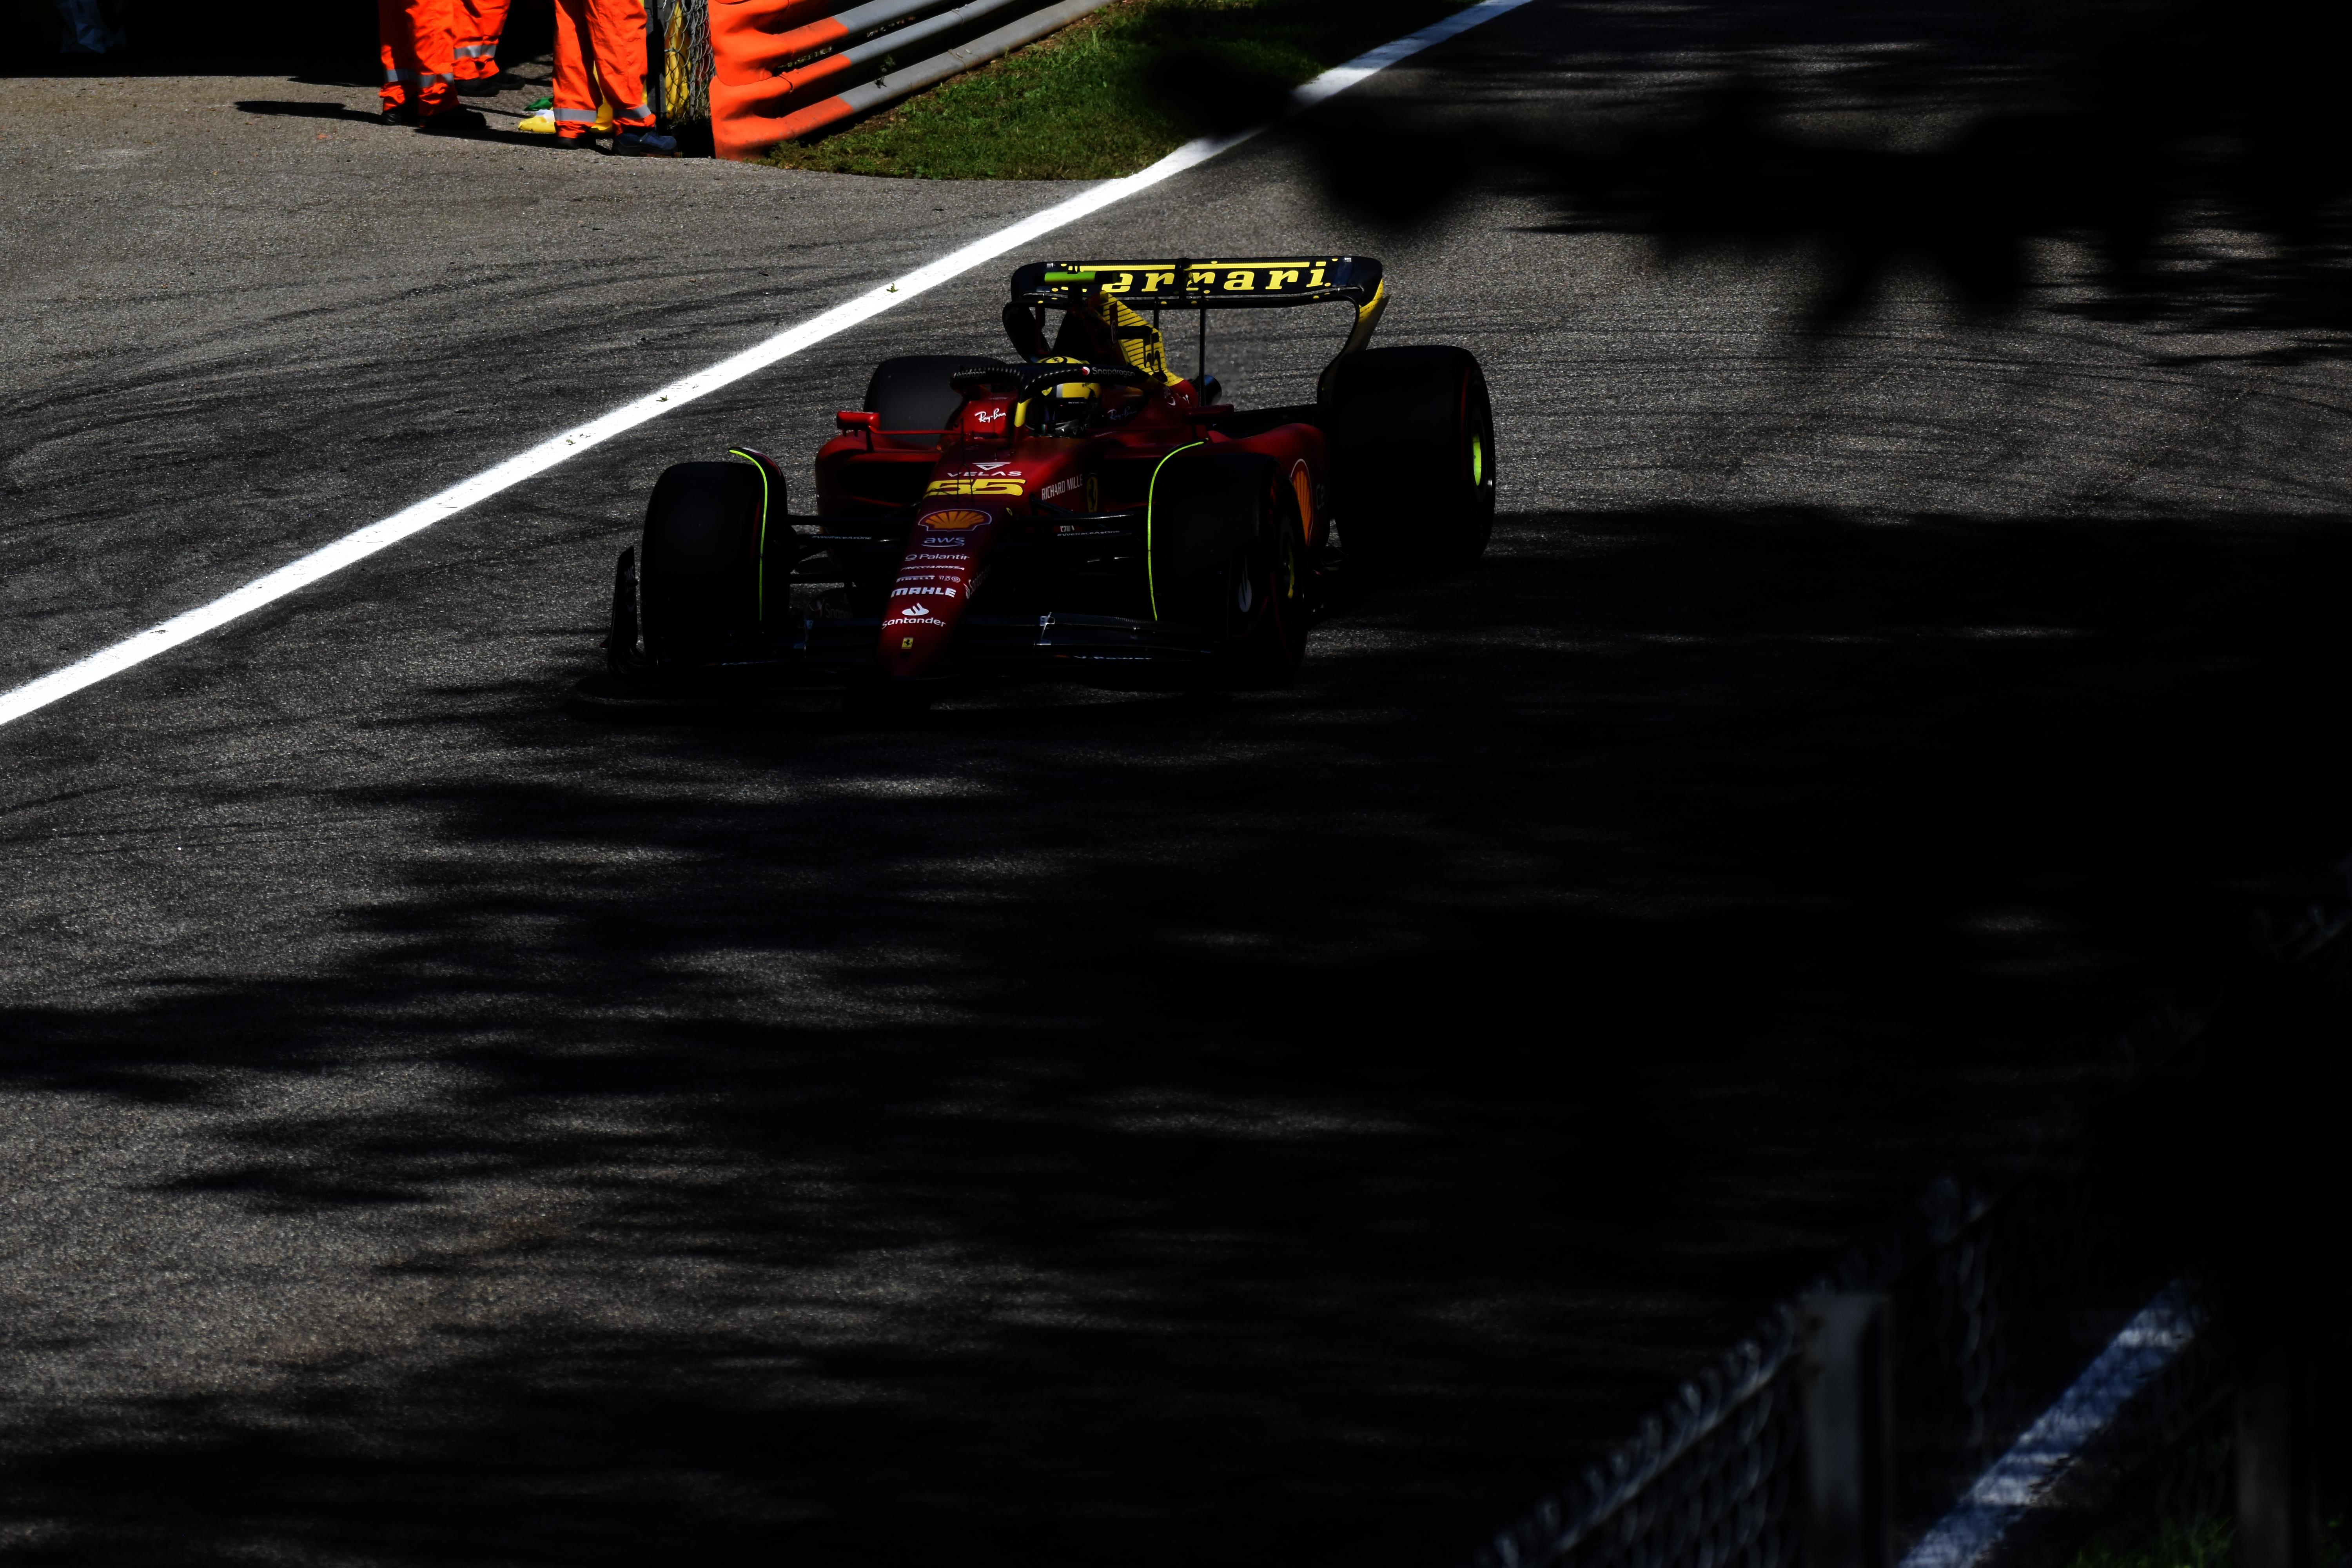
\includegraphics[width=\textwidth]{fig/out/1.ferrari_lin.jpg}
        \caption{$\texttt{ferrari\_lin.jpg}$. Linearized contrast}
    \end{subfigure}

    \begin{subfigure}{0.5\textwidth}
        \centering
        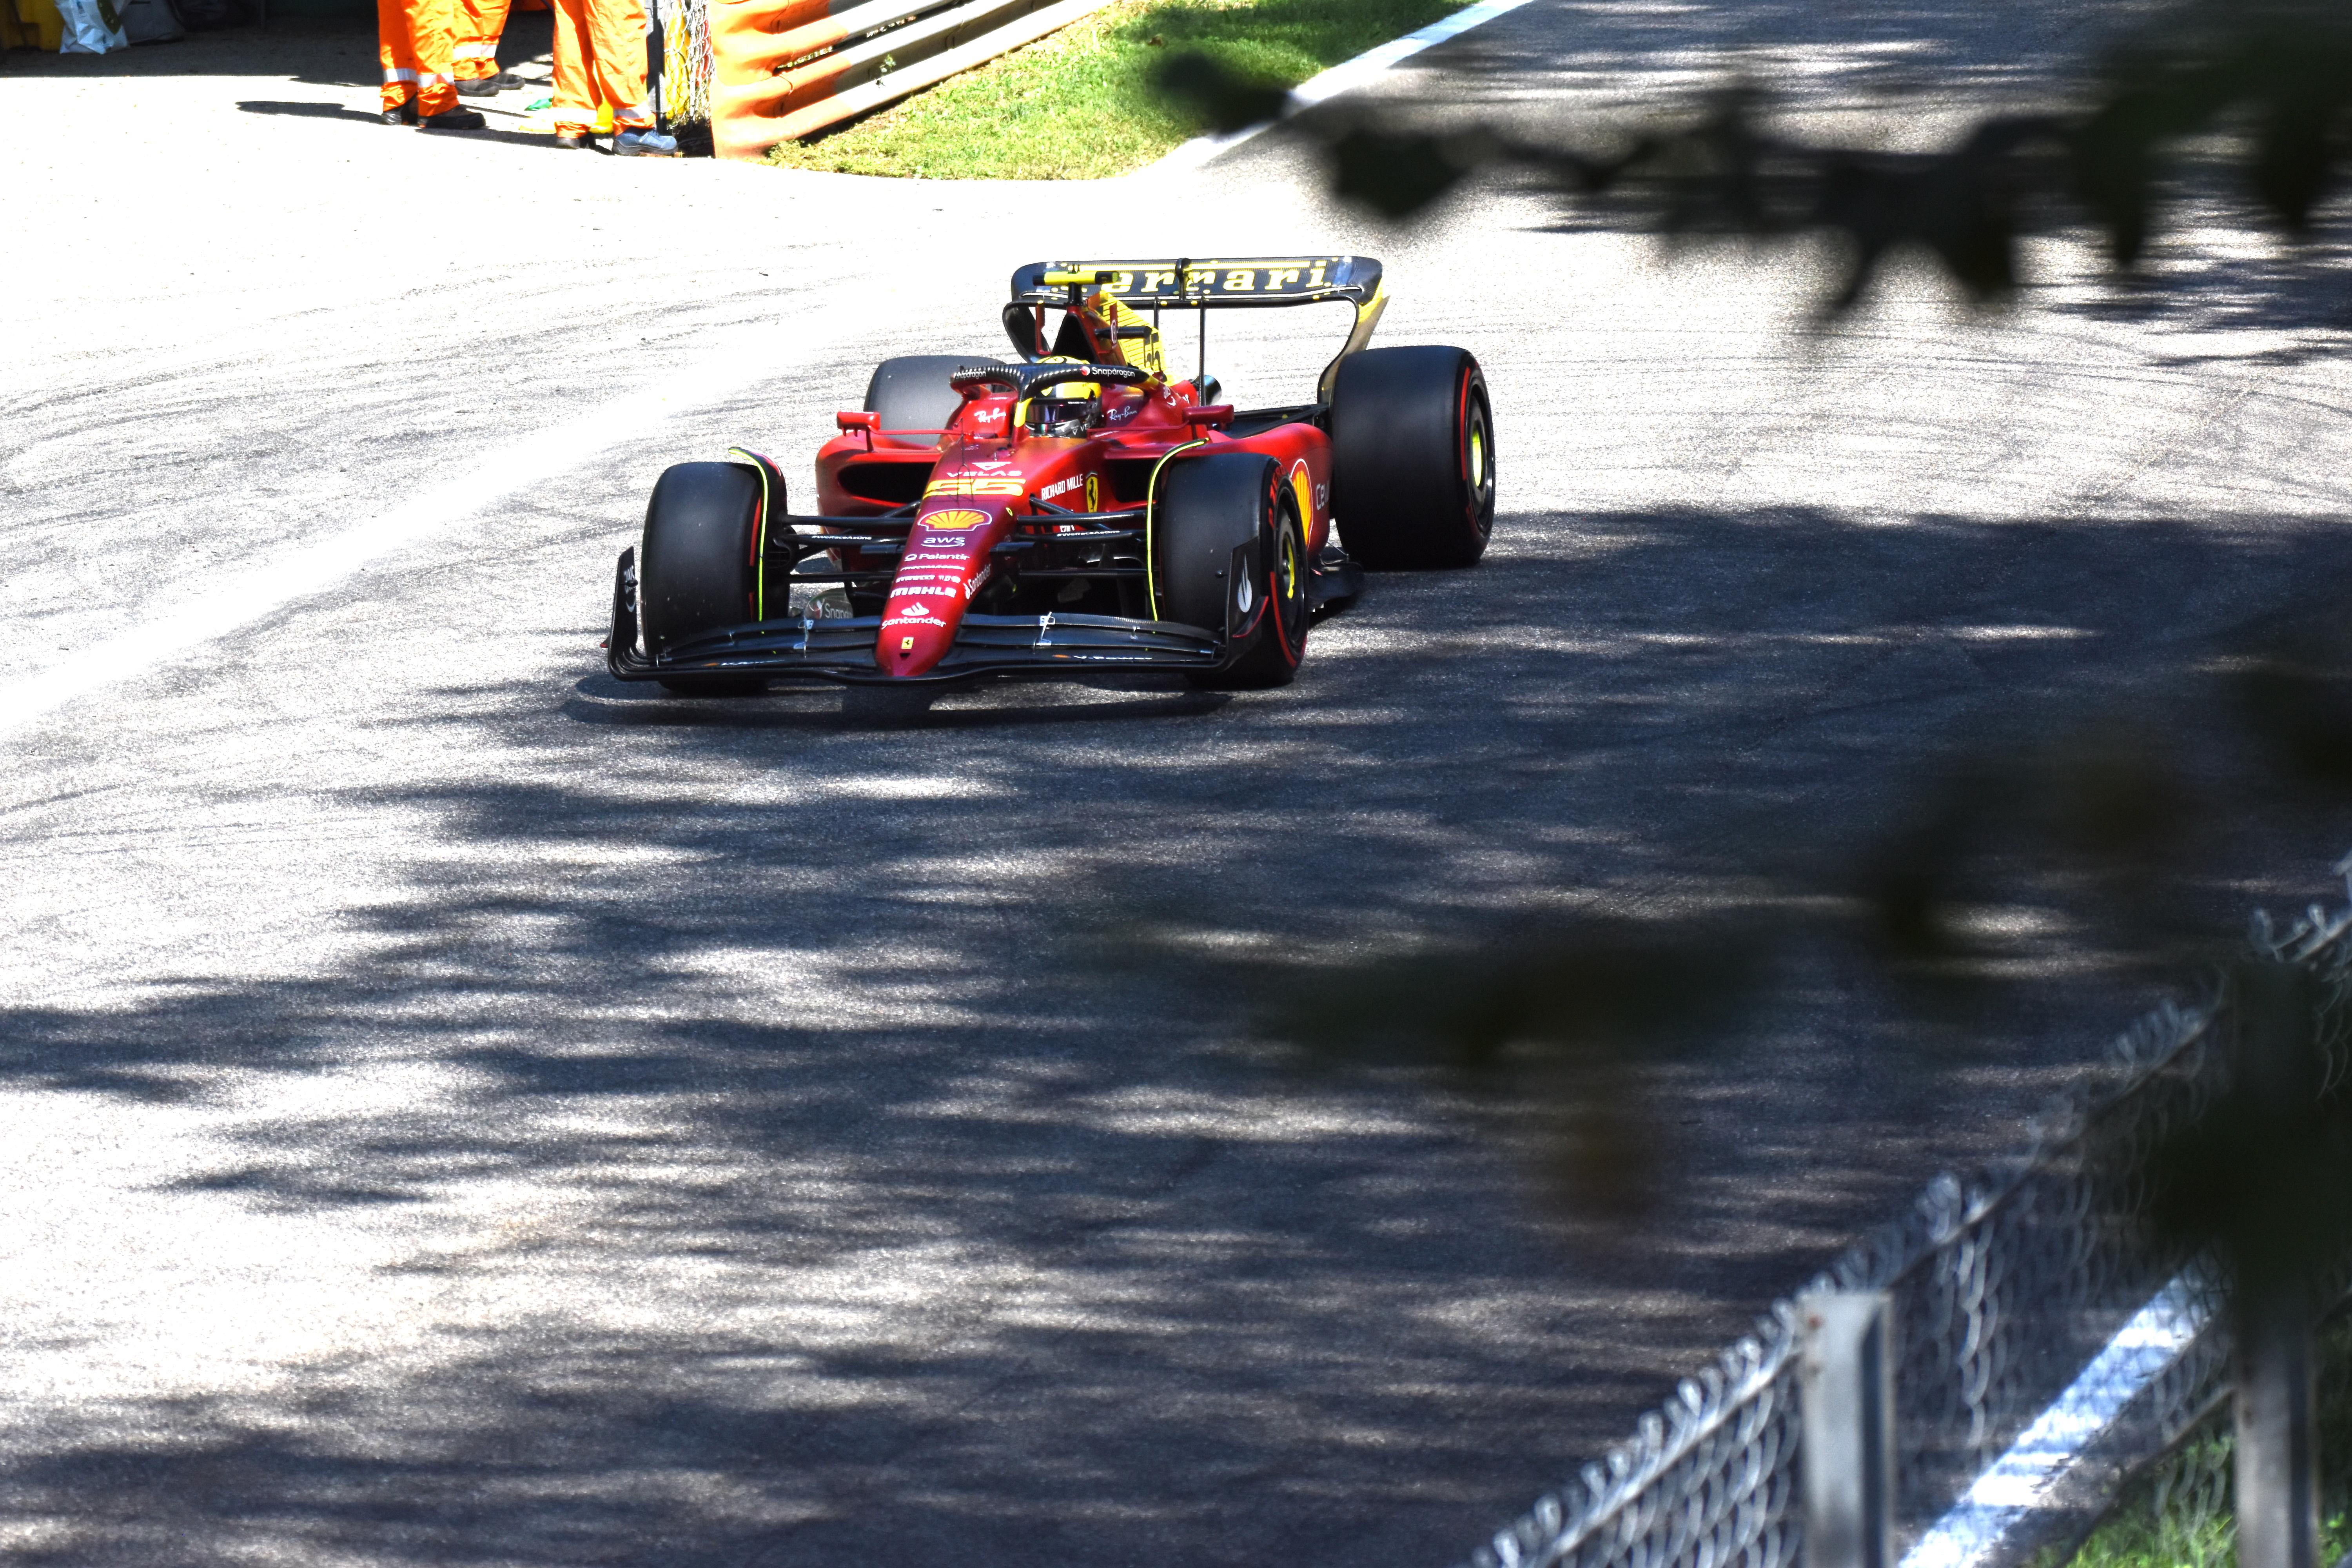
\includegraphics[width=\textwidth]{fig/out/1.ferrari_bri.jpg}
        \caption{$\texttt{ferrari\_bri.jpg}$. Scaled brightness}
    \end{subfigure}
    \begin{subfigure}{0.5\textwidth}
        \centering
        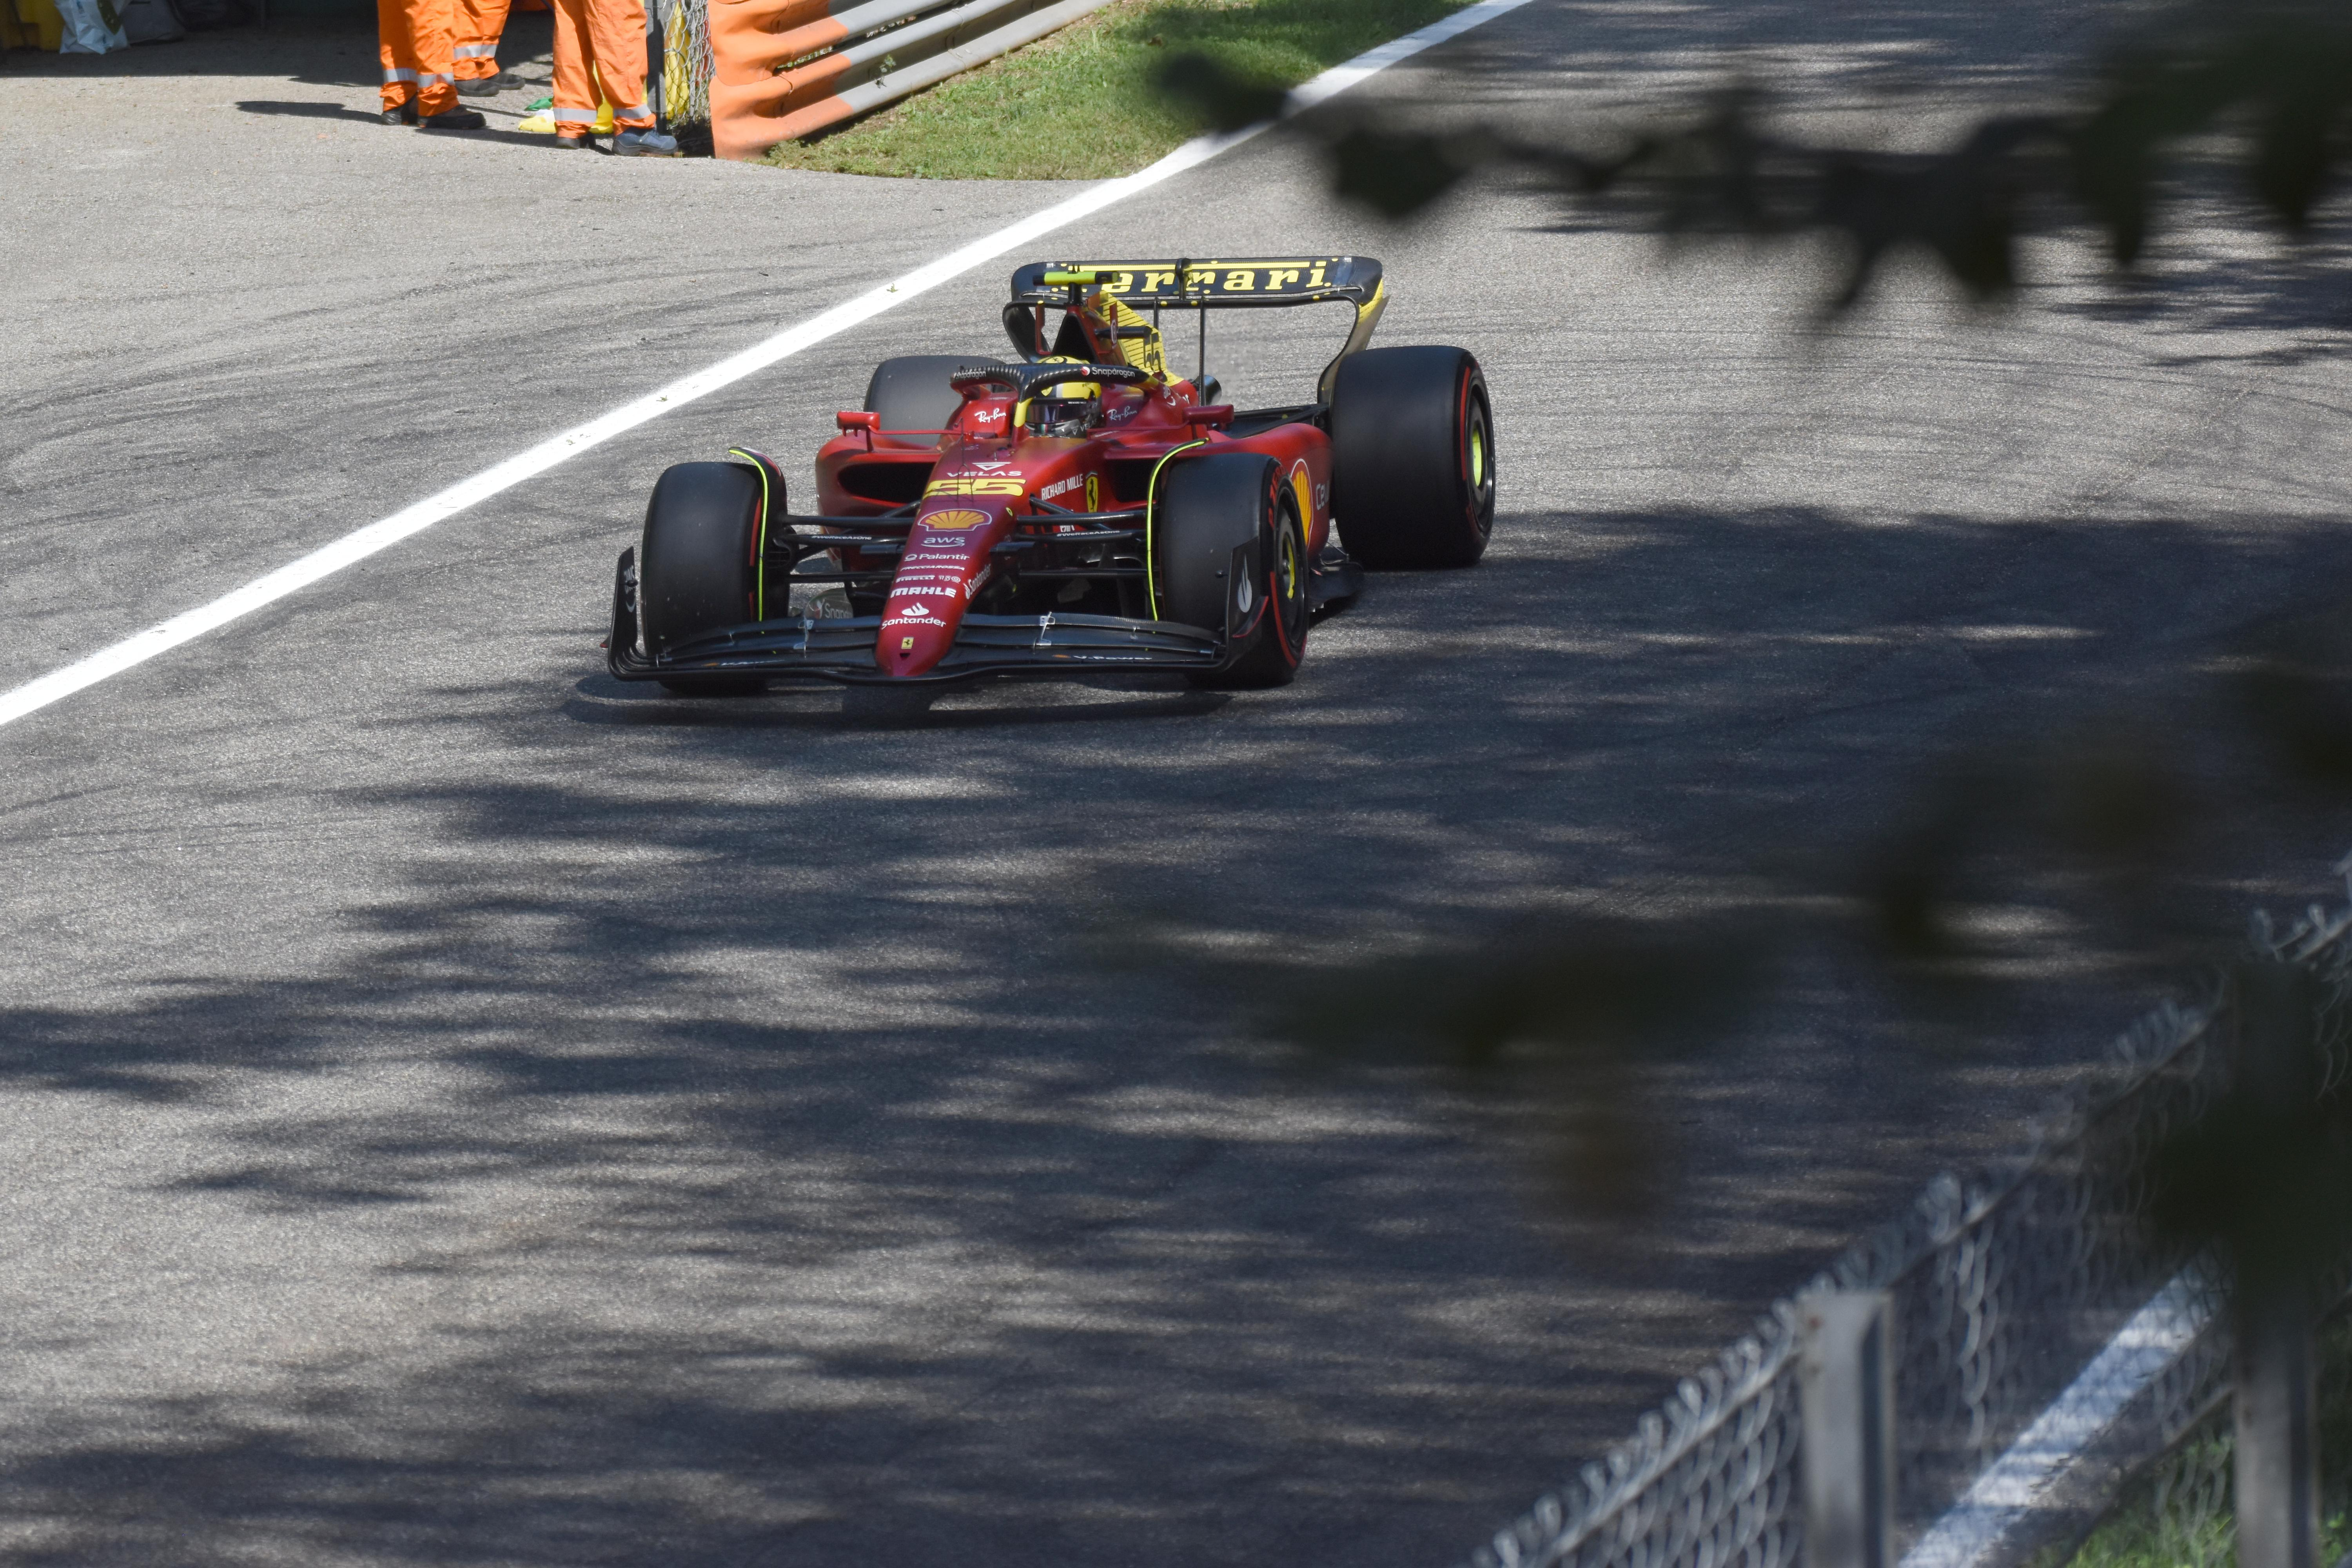
\includegraphics[width=\textwidth]{fig/out/1.ferrari_con.jpg}
        \caption{$\texttt {ferrari\_con.jpg}$. Exponential contrast.}
    \end{subfigure}

    \caption{Tonemapping procedure comparison.}
\end{figure}

\begin{figure}[h!]
    \begin{minted}[ frame=lines, framesep=2mm, linenos ]{matlab} 
im = imread("./media/ferrari.JPG");
im = double(im)./255;
imwrite(uint8(255.*im), "./out/1.ferrari.jpg");

% 1.1 Map pixels to 0-1 range and linearize image back
im_lin = im.^2.2;
imwrite(uint8(255.*im_lin), "./out/1.ferrari_lin.jpg");

% 1.2 Increase brightness
im_bri = im.*2;
imwrite(uint8(255.*im_bri), "./out/1.ferrari_bri.jpg");

% 1.3 Enhance contrast using exponential function
im_con = im.^0.7;
imwrite(uint8(255.*im_con), "./out/1.ferrari_con.jpg");
figure()
imshow([im, im_lin,im_bri,im_con], []);
        \end{minted}
\caption{Matlab code performing various intensity transformations on the image $\texttt{ferrari.jpg}$.}
\end{figure}
\subsection{Color correction [4 points]}
\begin{figure}[h!]
    \begin{subfigure}{0.33\linewidth}
        \centering
        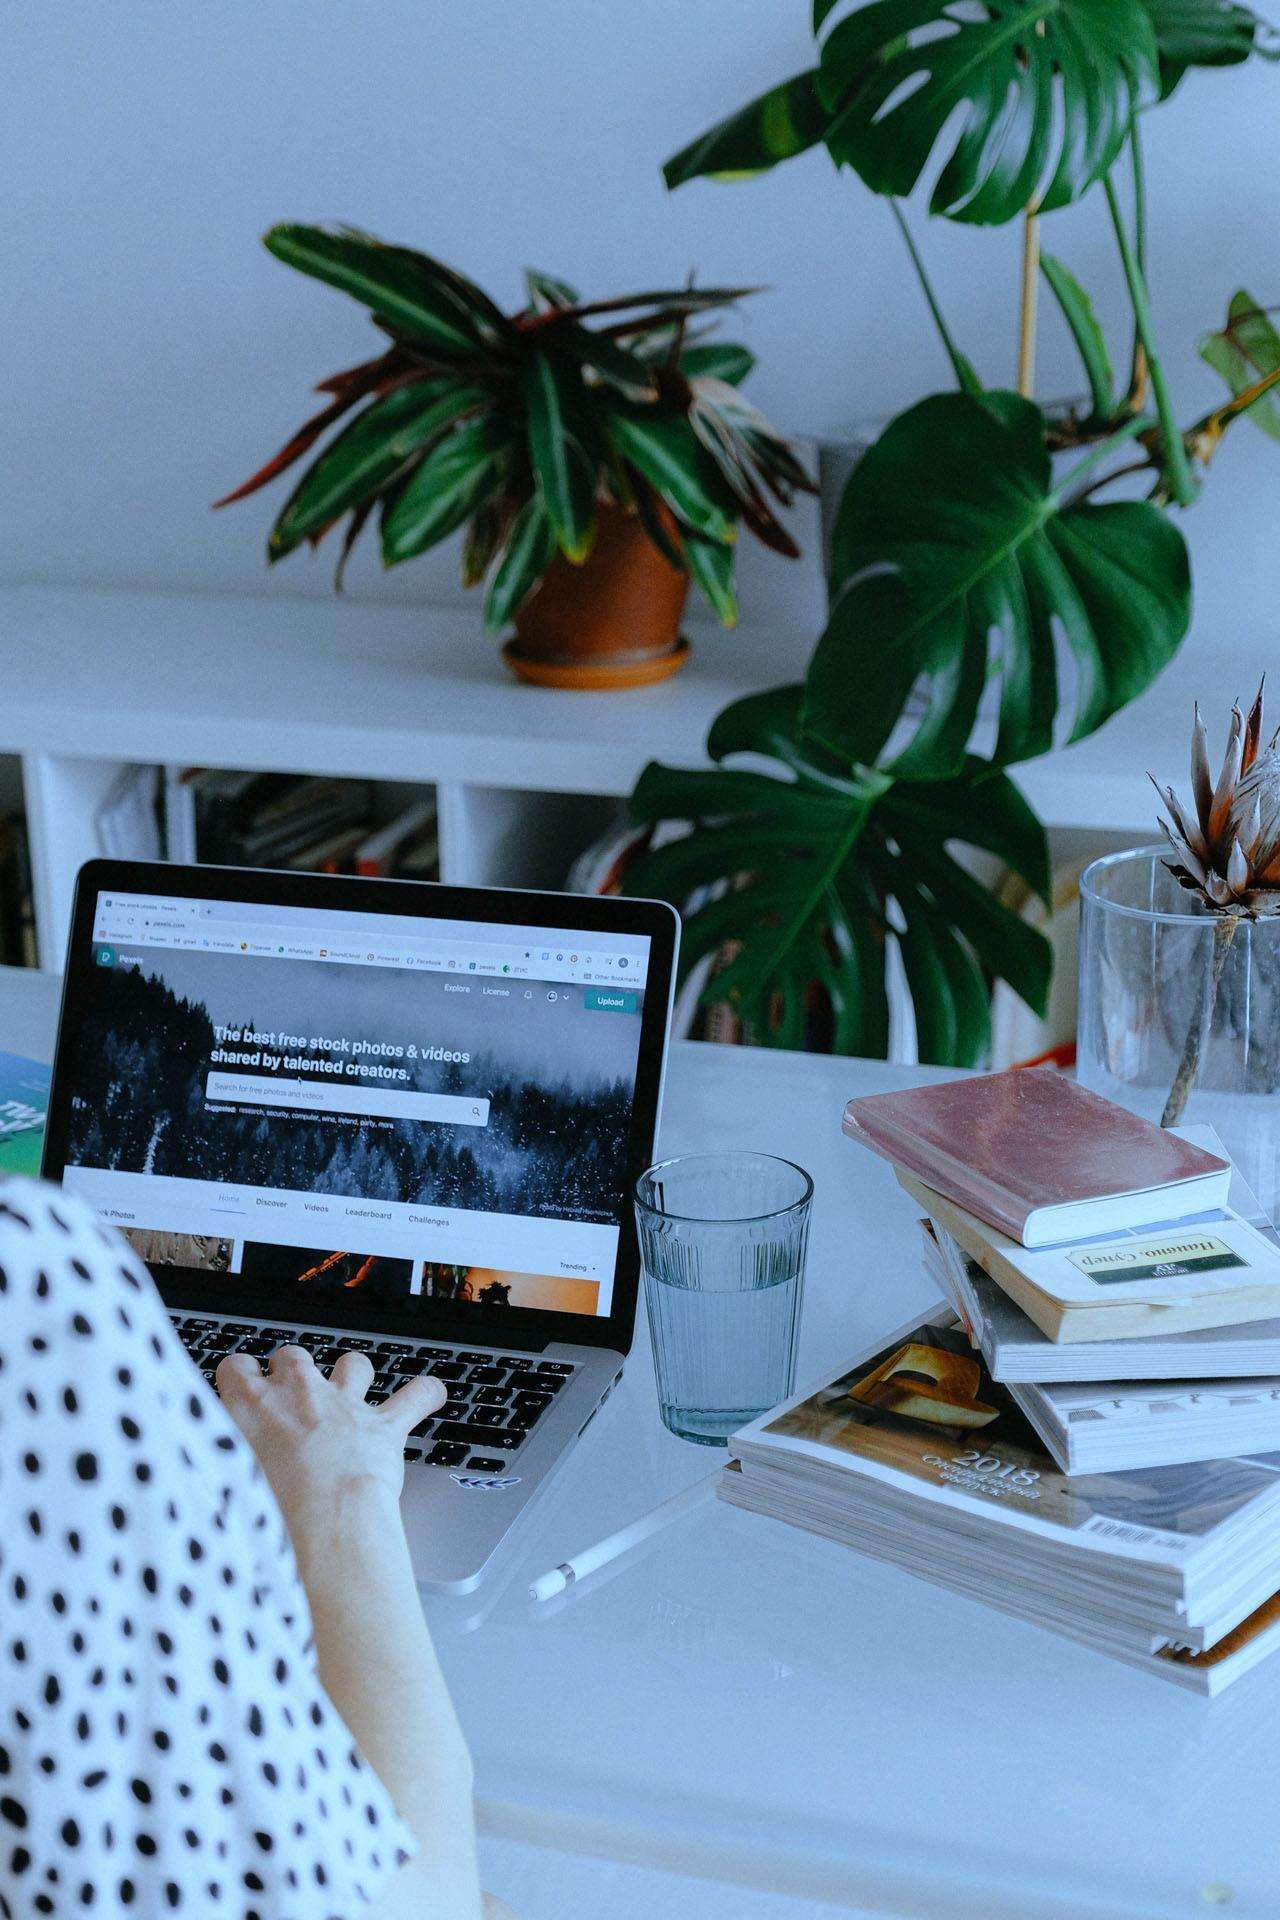
\includegraphics[width=\linewidth]{fig/out/2.wb.jpg}
        \caption{Original image}
    \end{subfigure}
    \begin{subfigure}{0.33\linewidth}
        \centering
        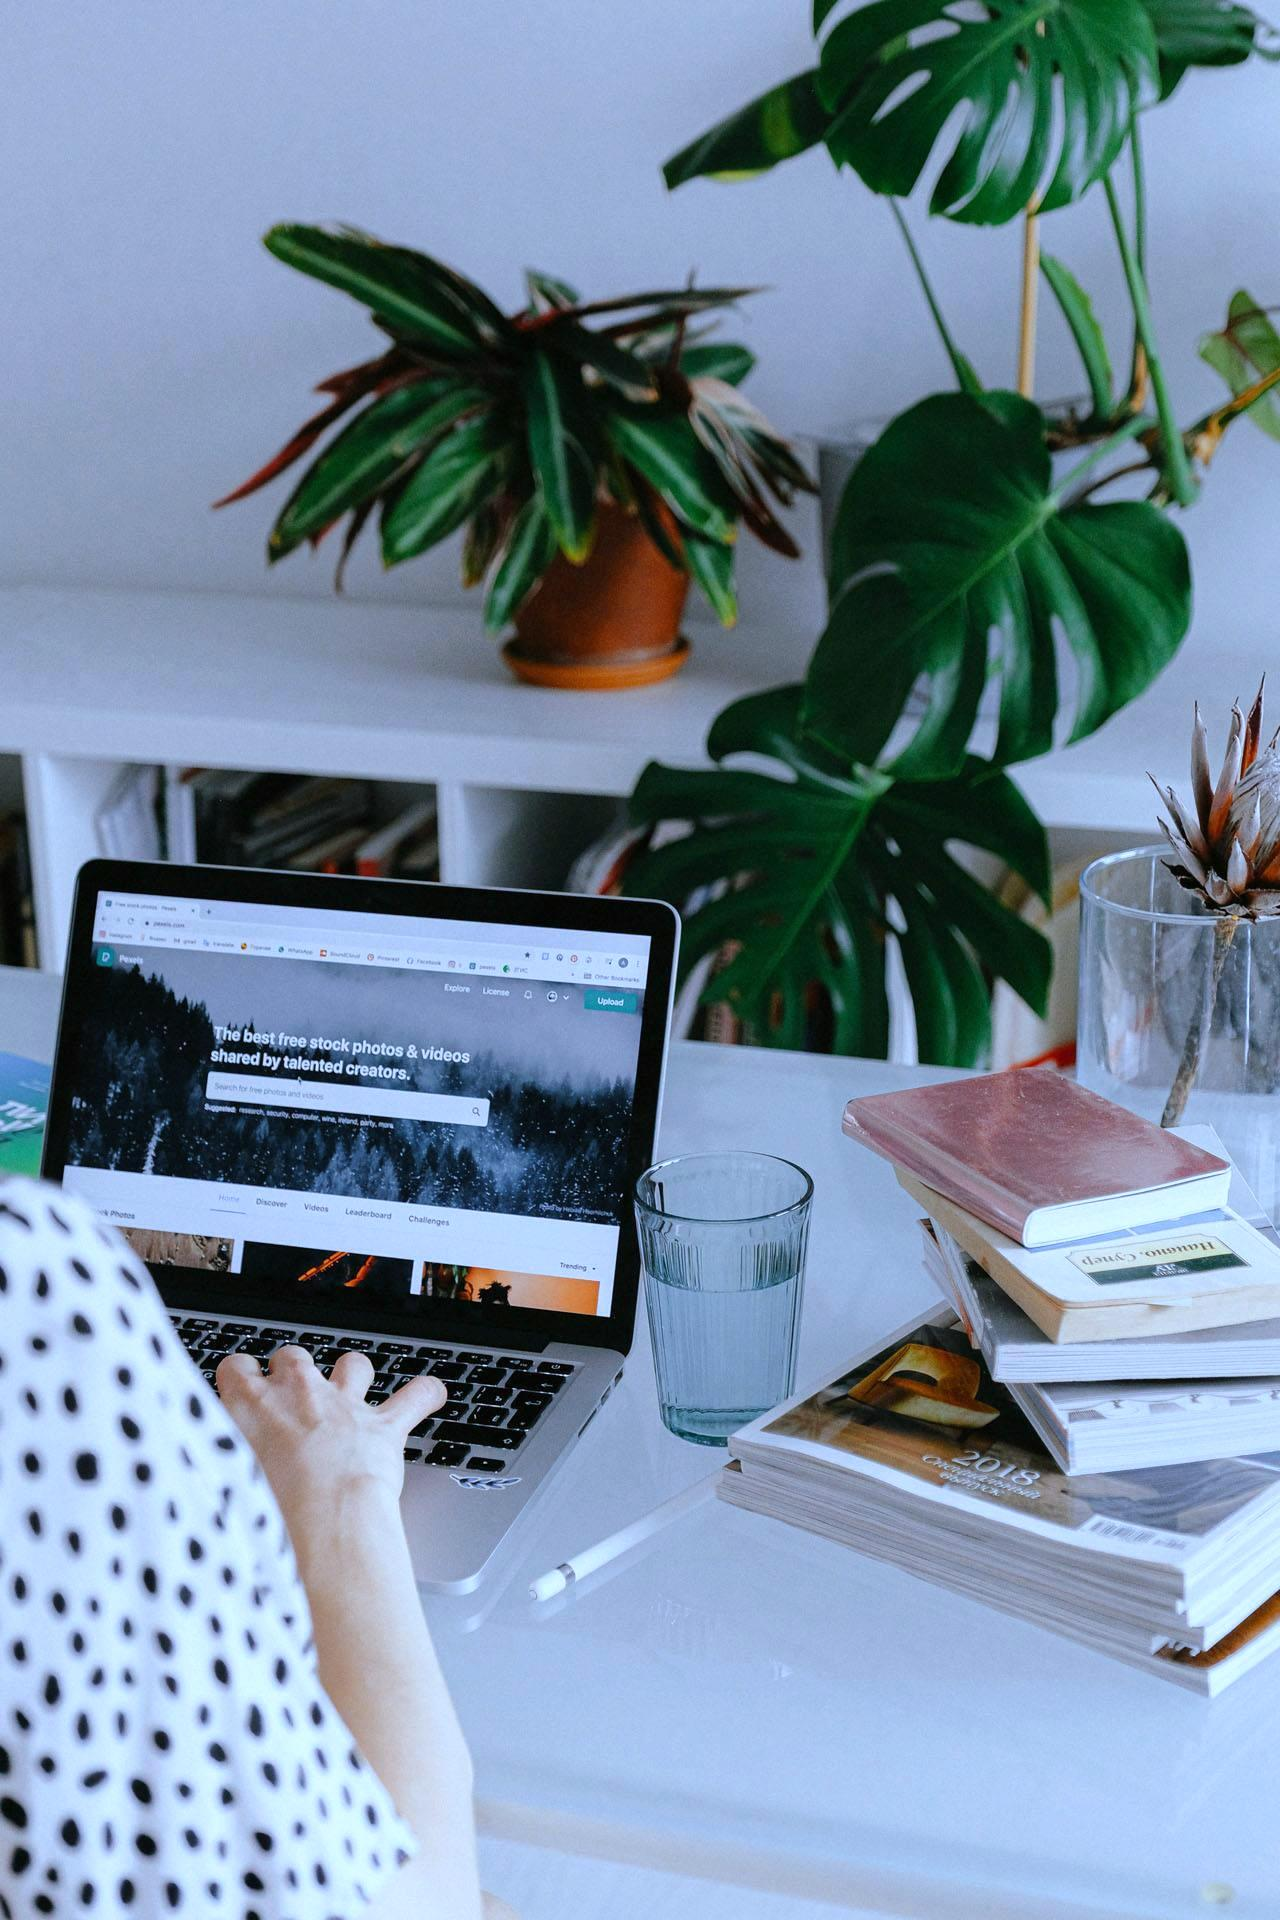
\includegraphics[width=\linewidth]{fig/out/2.wb_pxcorr.jpg}
        \caption{Pixel-based correction}
    \end{subfigure}
    \begin{subfigure}{0.33\linewidth}
        \centering
        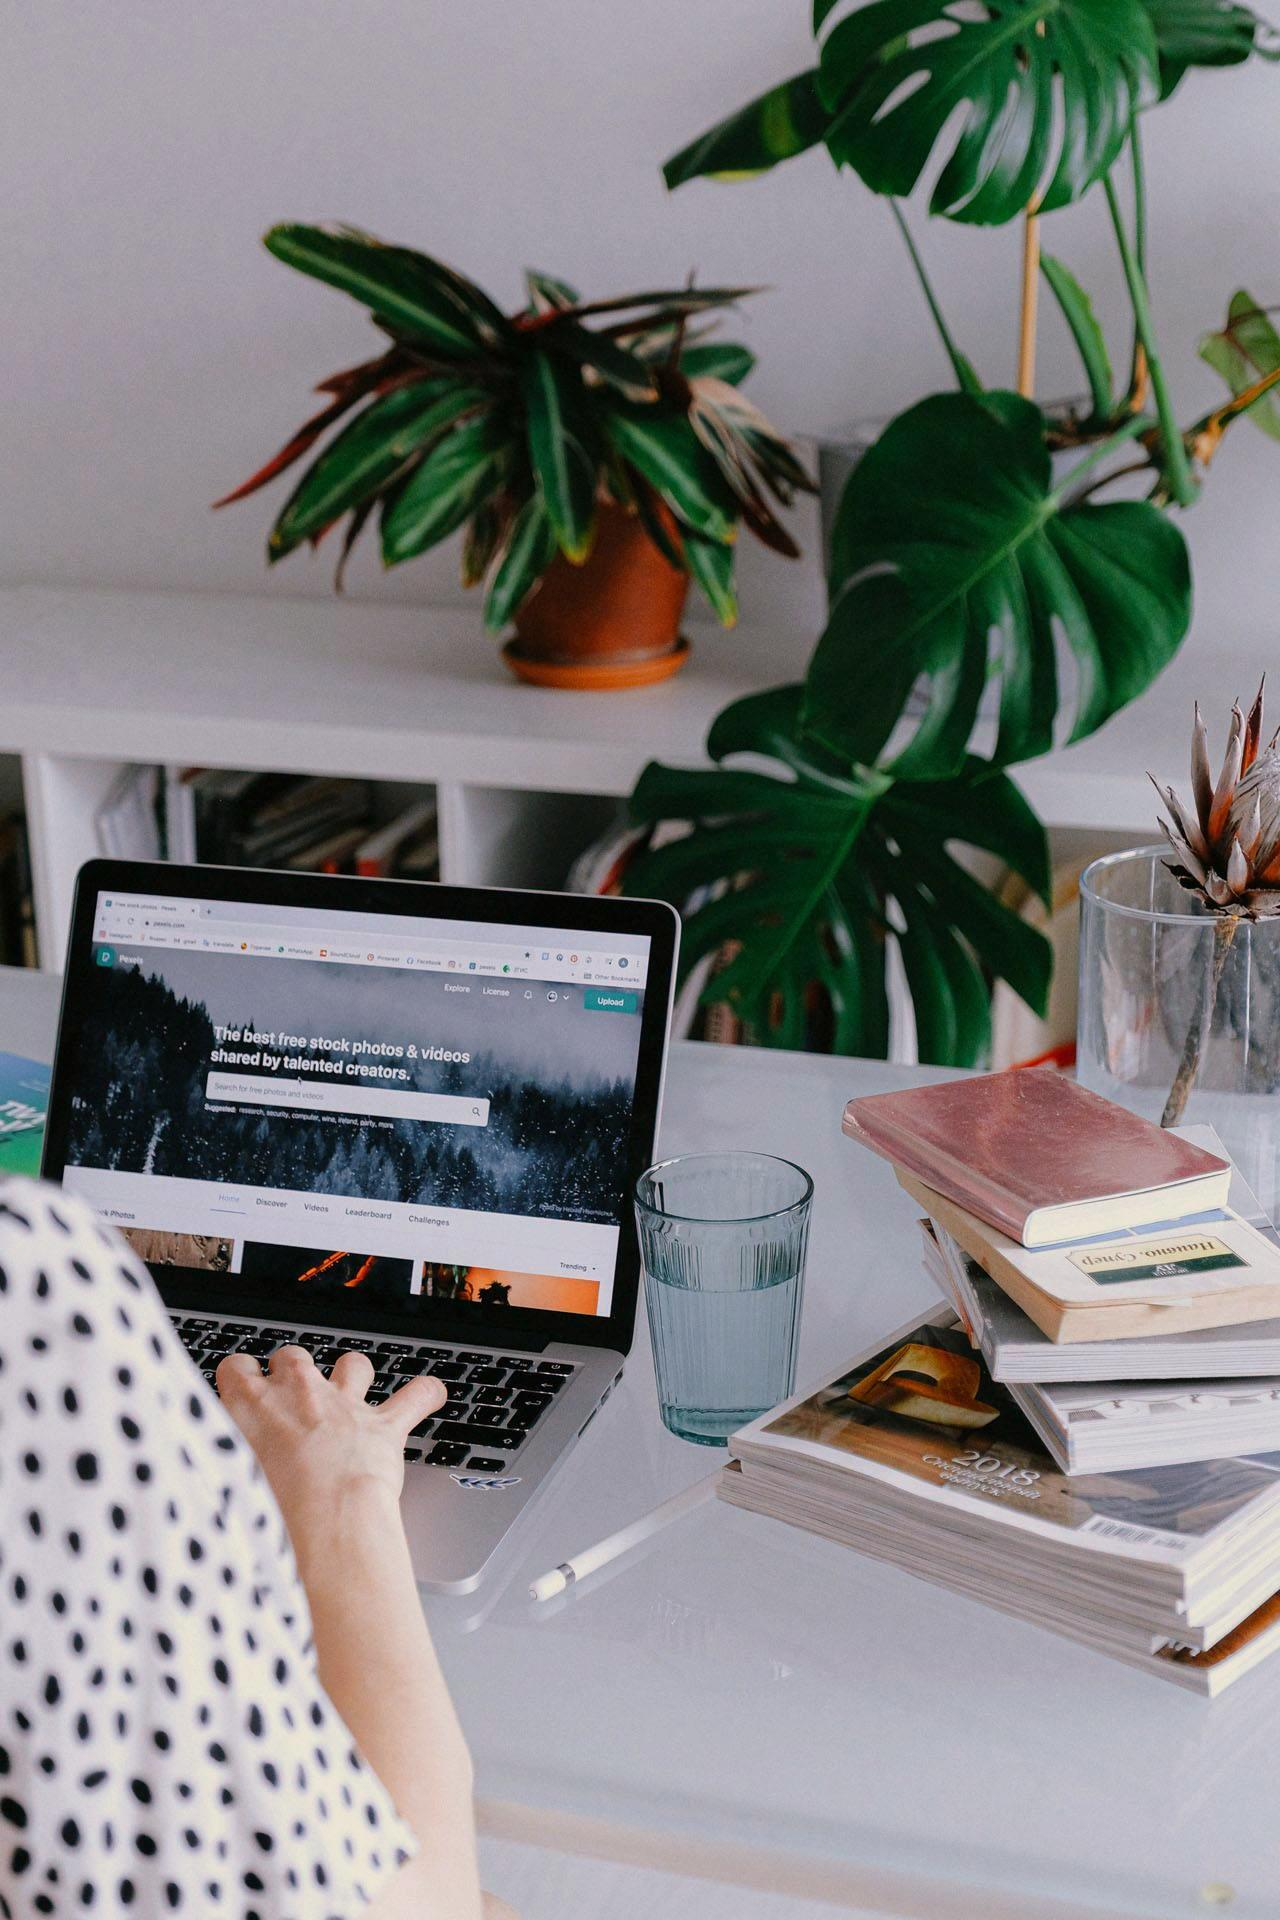
\includegraphics[width=\linewidth]{fig/out/2.wb_gwa.jpg}
        \caption{Gray-world assumption correction}
    \end{subfigure}
    \caption{Color correction procedures comparison.}
\end{figure}

\begin{figure}[h!]
    \begin{minted}[ frame=lines, framesep=2mm, linenos ]{matlab} 
im = imread("./media/white_balance_input.jpg");
im = (double(im)./255);
imwrite(uint8(255.*im), "./out/2.wb.jpg");

channelmean = mean(mean(im))
% 2.1 Pixel-based correction
figure()
imshow(im);
coords = int32(ginput(1));
px_color = im(coords(2), coords(1), 1:3);
gain = px_color./channelmean;
im_pxcorr = im.*gain;
imwrite(uint8(255.*im_pxcorr), "./out/2.wb_pxcorr.jpg");

% 2.2 Gray-world assumption
gain = 0.5./channelmean;
im_gwa = im.*gain;
imwrite(uint8(255.*im_gwa), "./out/2.wb_gwa.jpg");

figure()
imshow([im, im_pxcorr, im_gwa])
        \end{minted}
\caption{Matlab code performing various intensity transformations on the image $\texttt{ferrari.jpg}$.}
\end{figure}

\subsection{Histograms [1 point]}
\begin{figure}[h!]
    \centering
    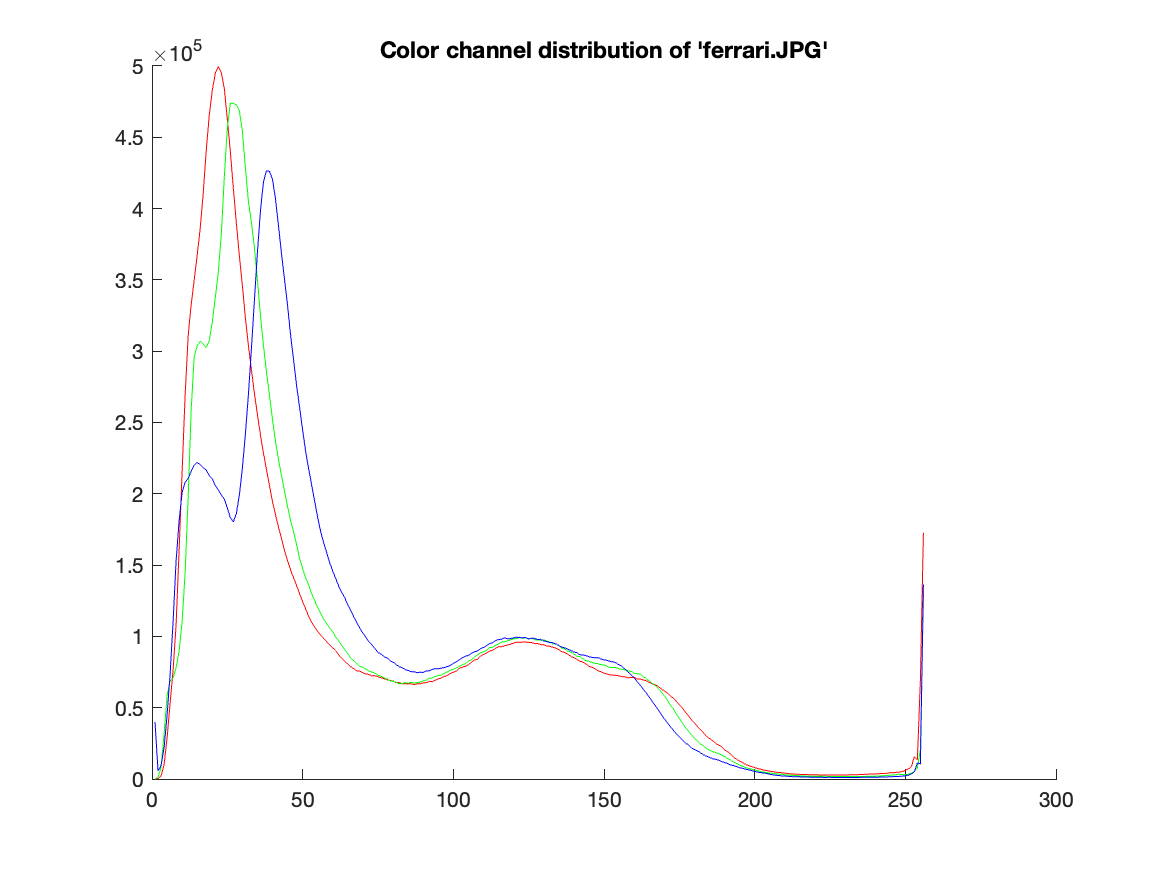
\includegraphics[width=\linewidth]{fig/out/3.histogram.png}
    \caption{Color channel distribution of the image $\texttt{ferrari.JPG}$.}
\end{figure}

\subsection{Histogram Equalization [5 points + 2 Bonus]}


\subsection{Manual histogram equalization [2 points]}


\subsection{Thresholding \& matting [4 points]}

\begin{figure}[h!]
    \begin{subfigure}{0.33\textwidth}
        \centering
        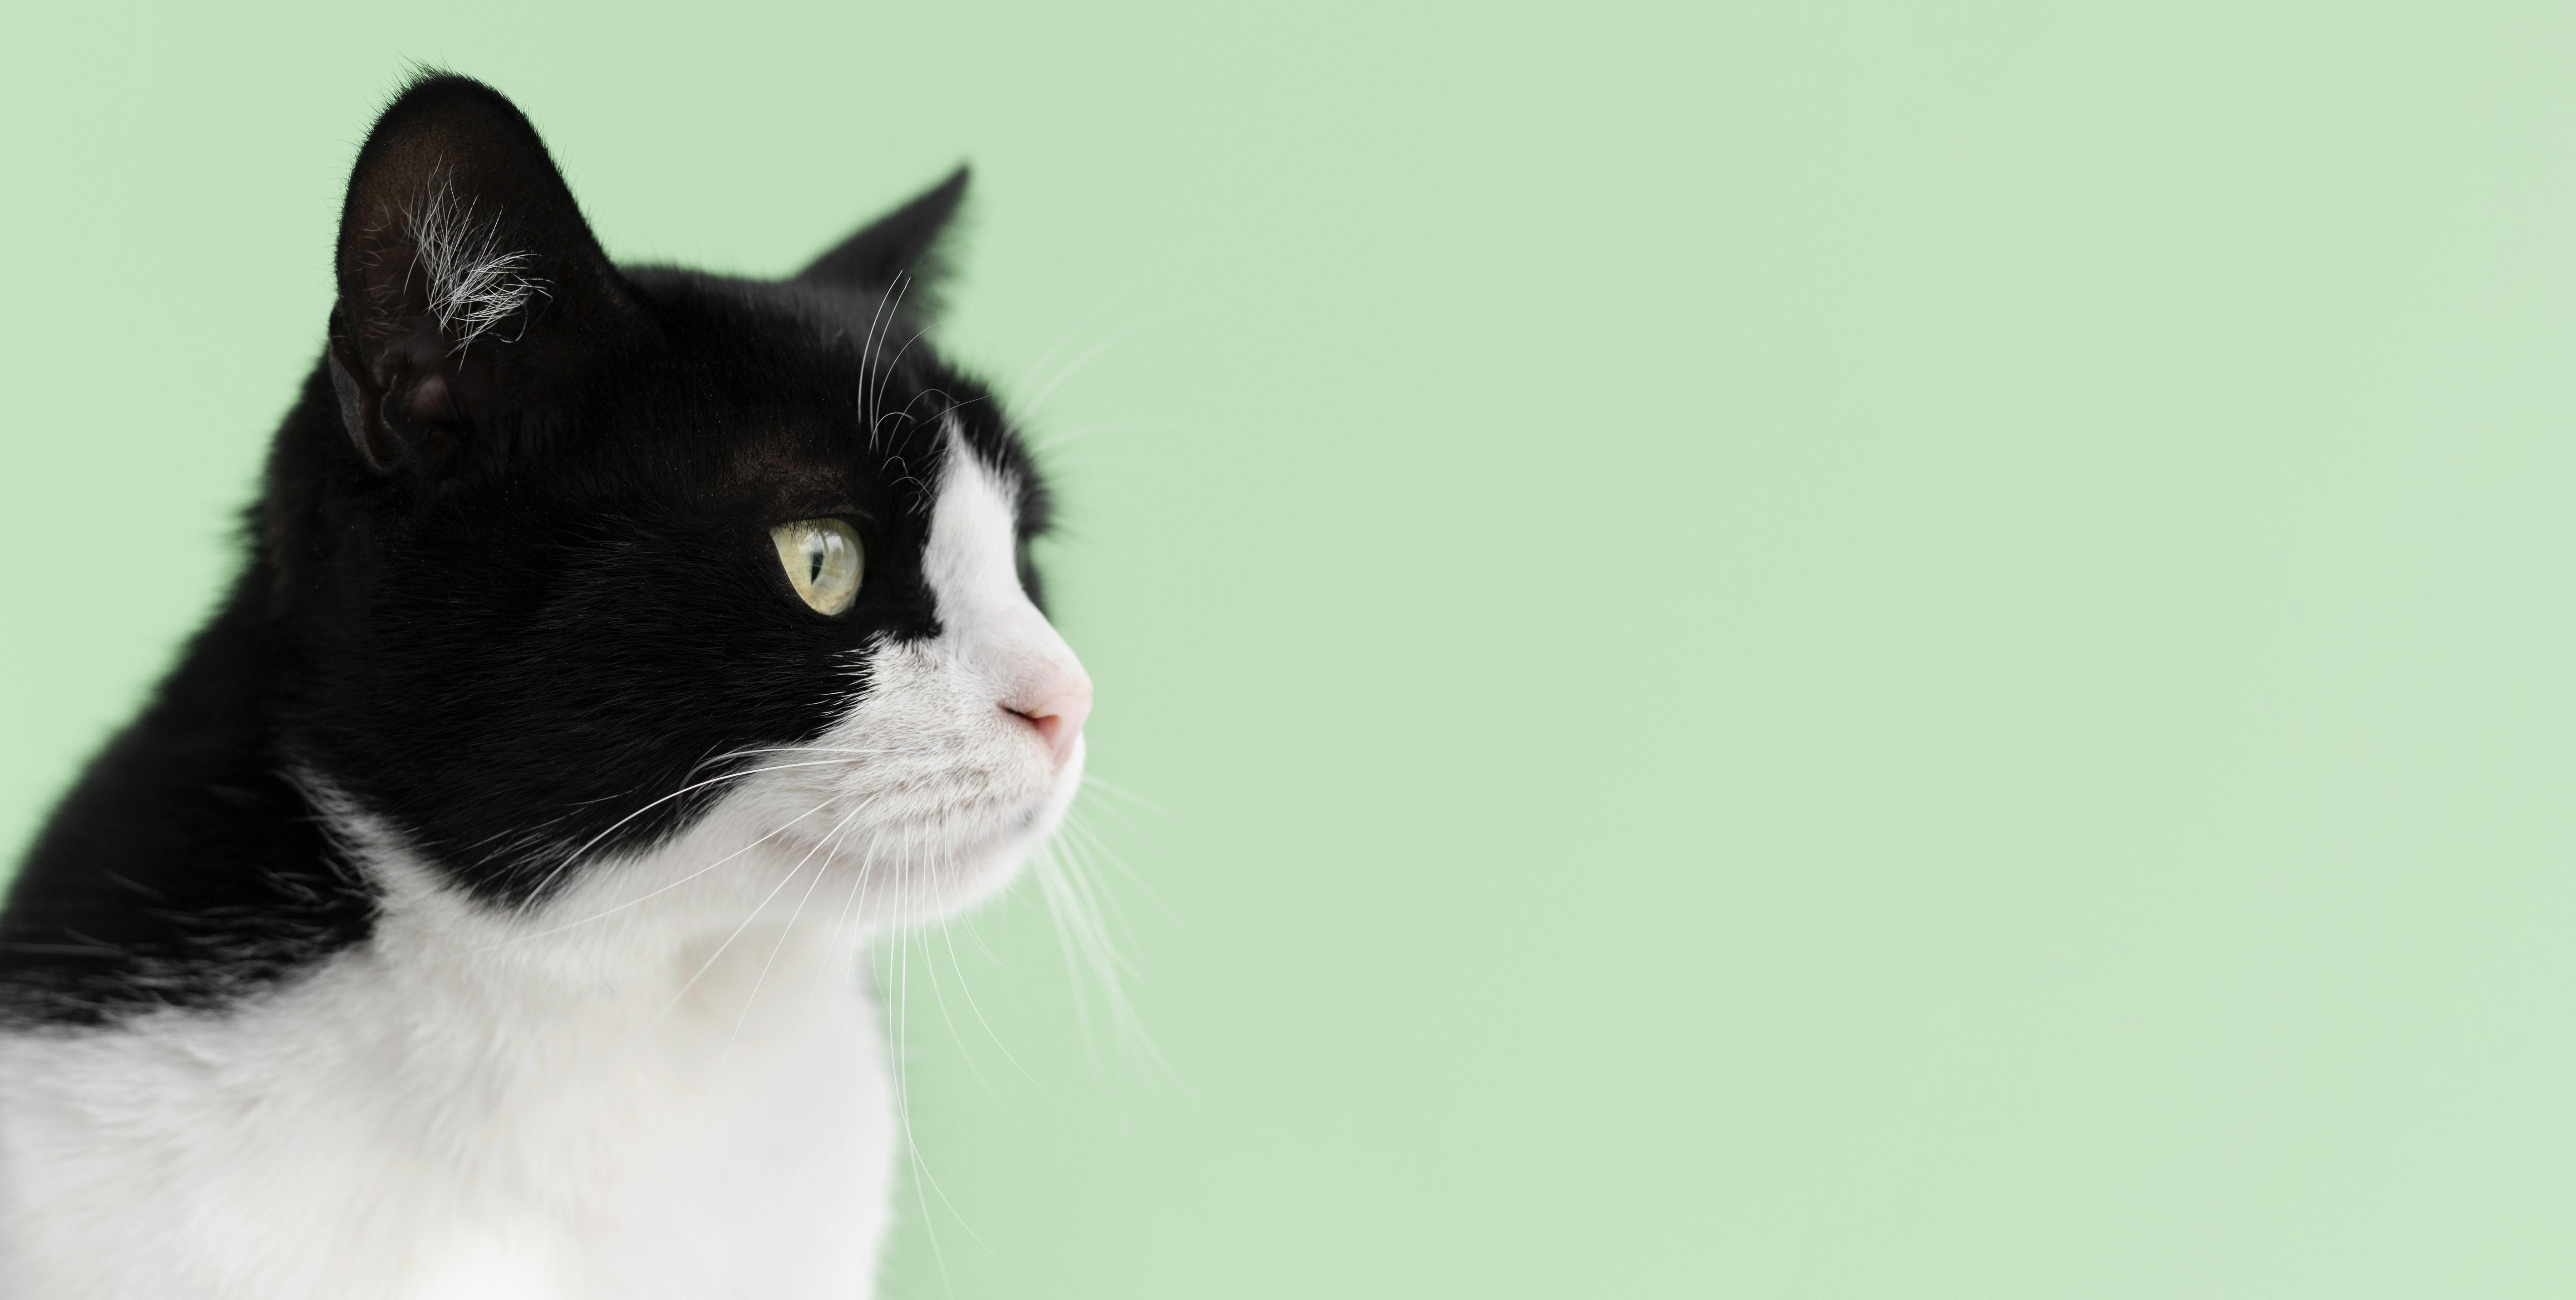
\includegraphics[width=\textwidth]{fig/out/6.cat.jpg}
        \caption{Original image.}
    \end{subfigure}
    \begin{subfigure}{0.33\textwidth}
        \centering
        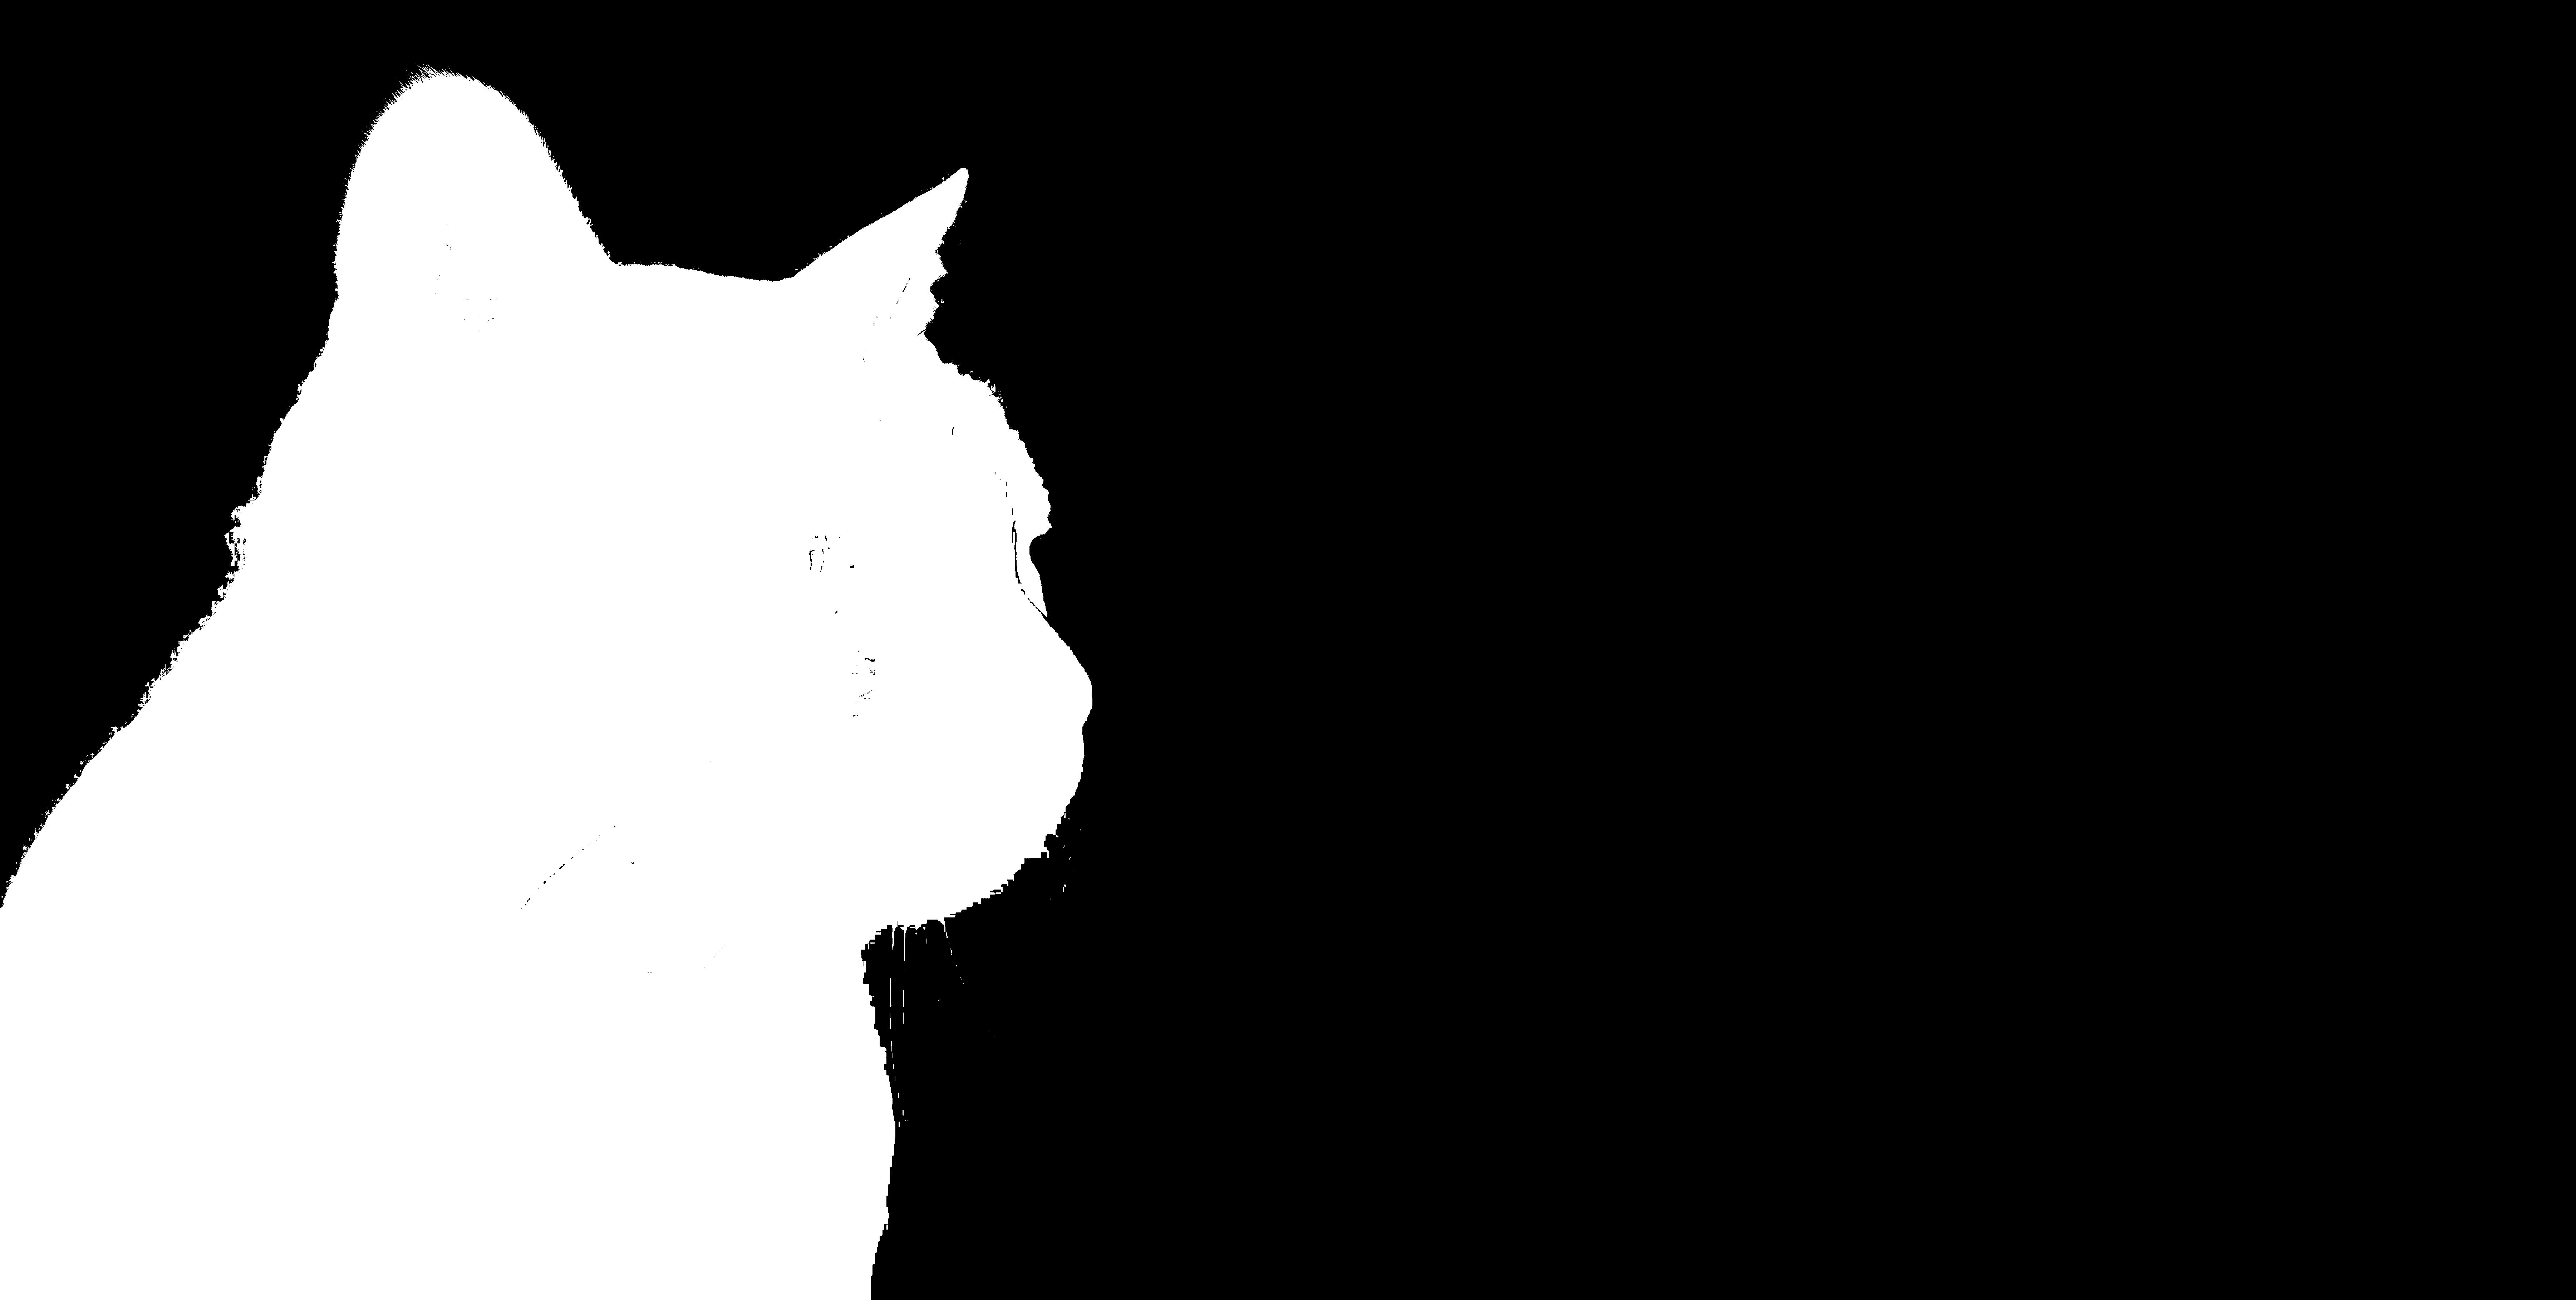
\includegraphics[width=\textwidth]{fig/out/6.mask.jpg}
        \caption{Chroma Key mask.}
    \end{subfigure}
    \begin{subfigure}{0.33\textwidth}
        \centering
        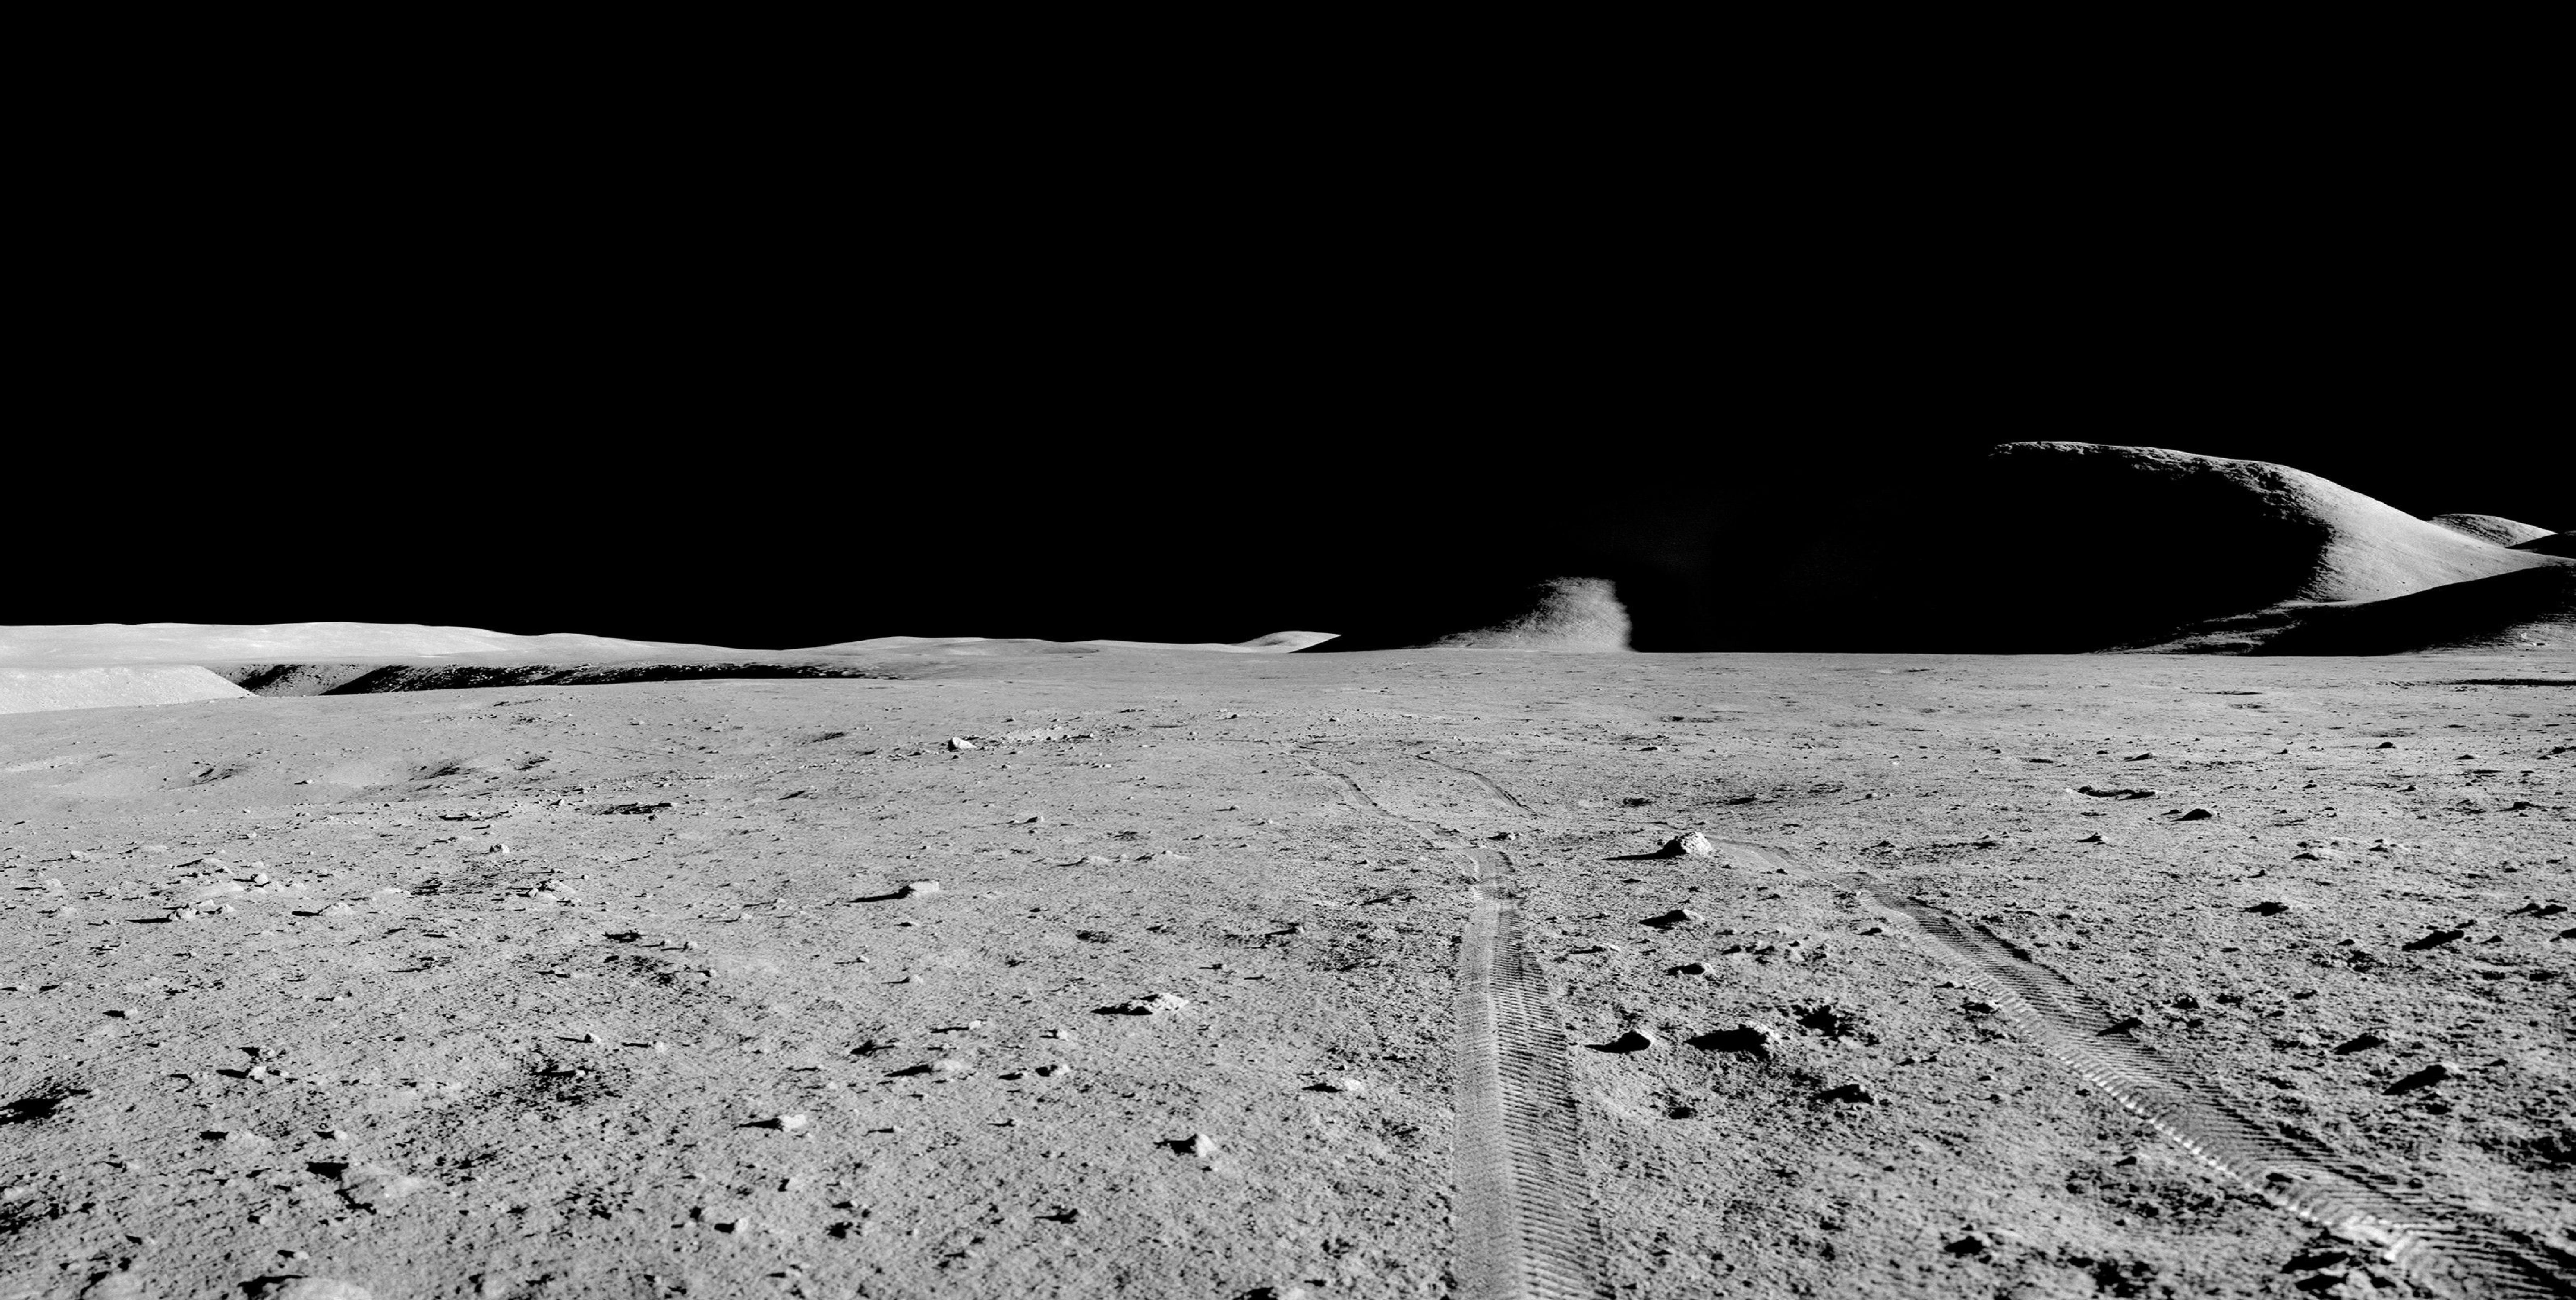
\includegraphics[width=\textwidth]{fig/out/6.spacebg.jpg}
        \caption{Background image.}
    \end{subfigure}

    \begin{subfigure}{1\textwidth}
        \centering
        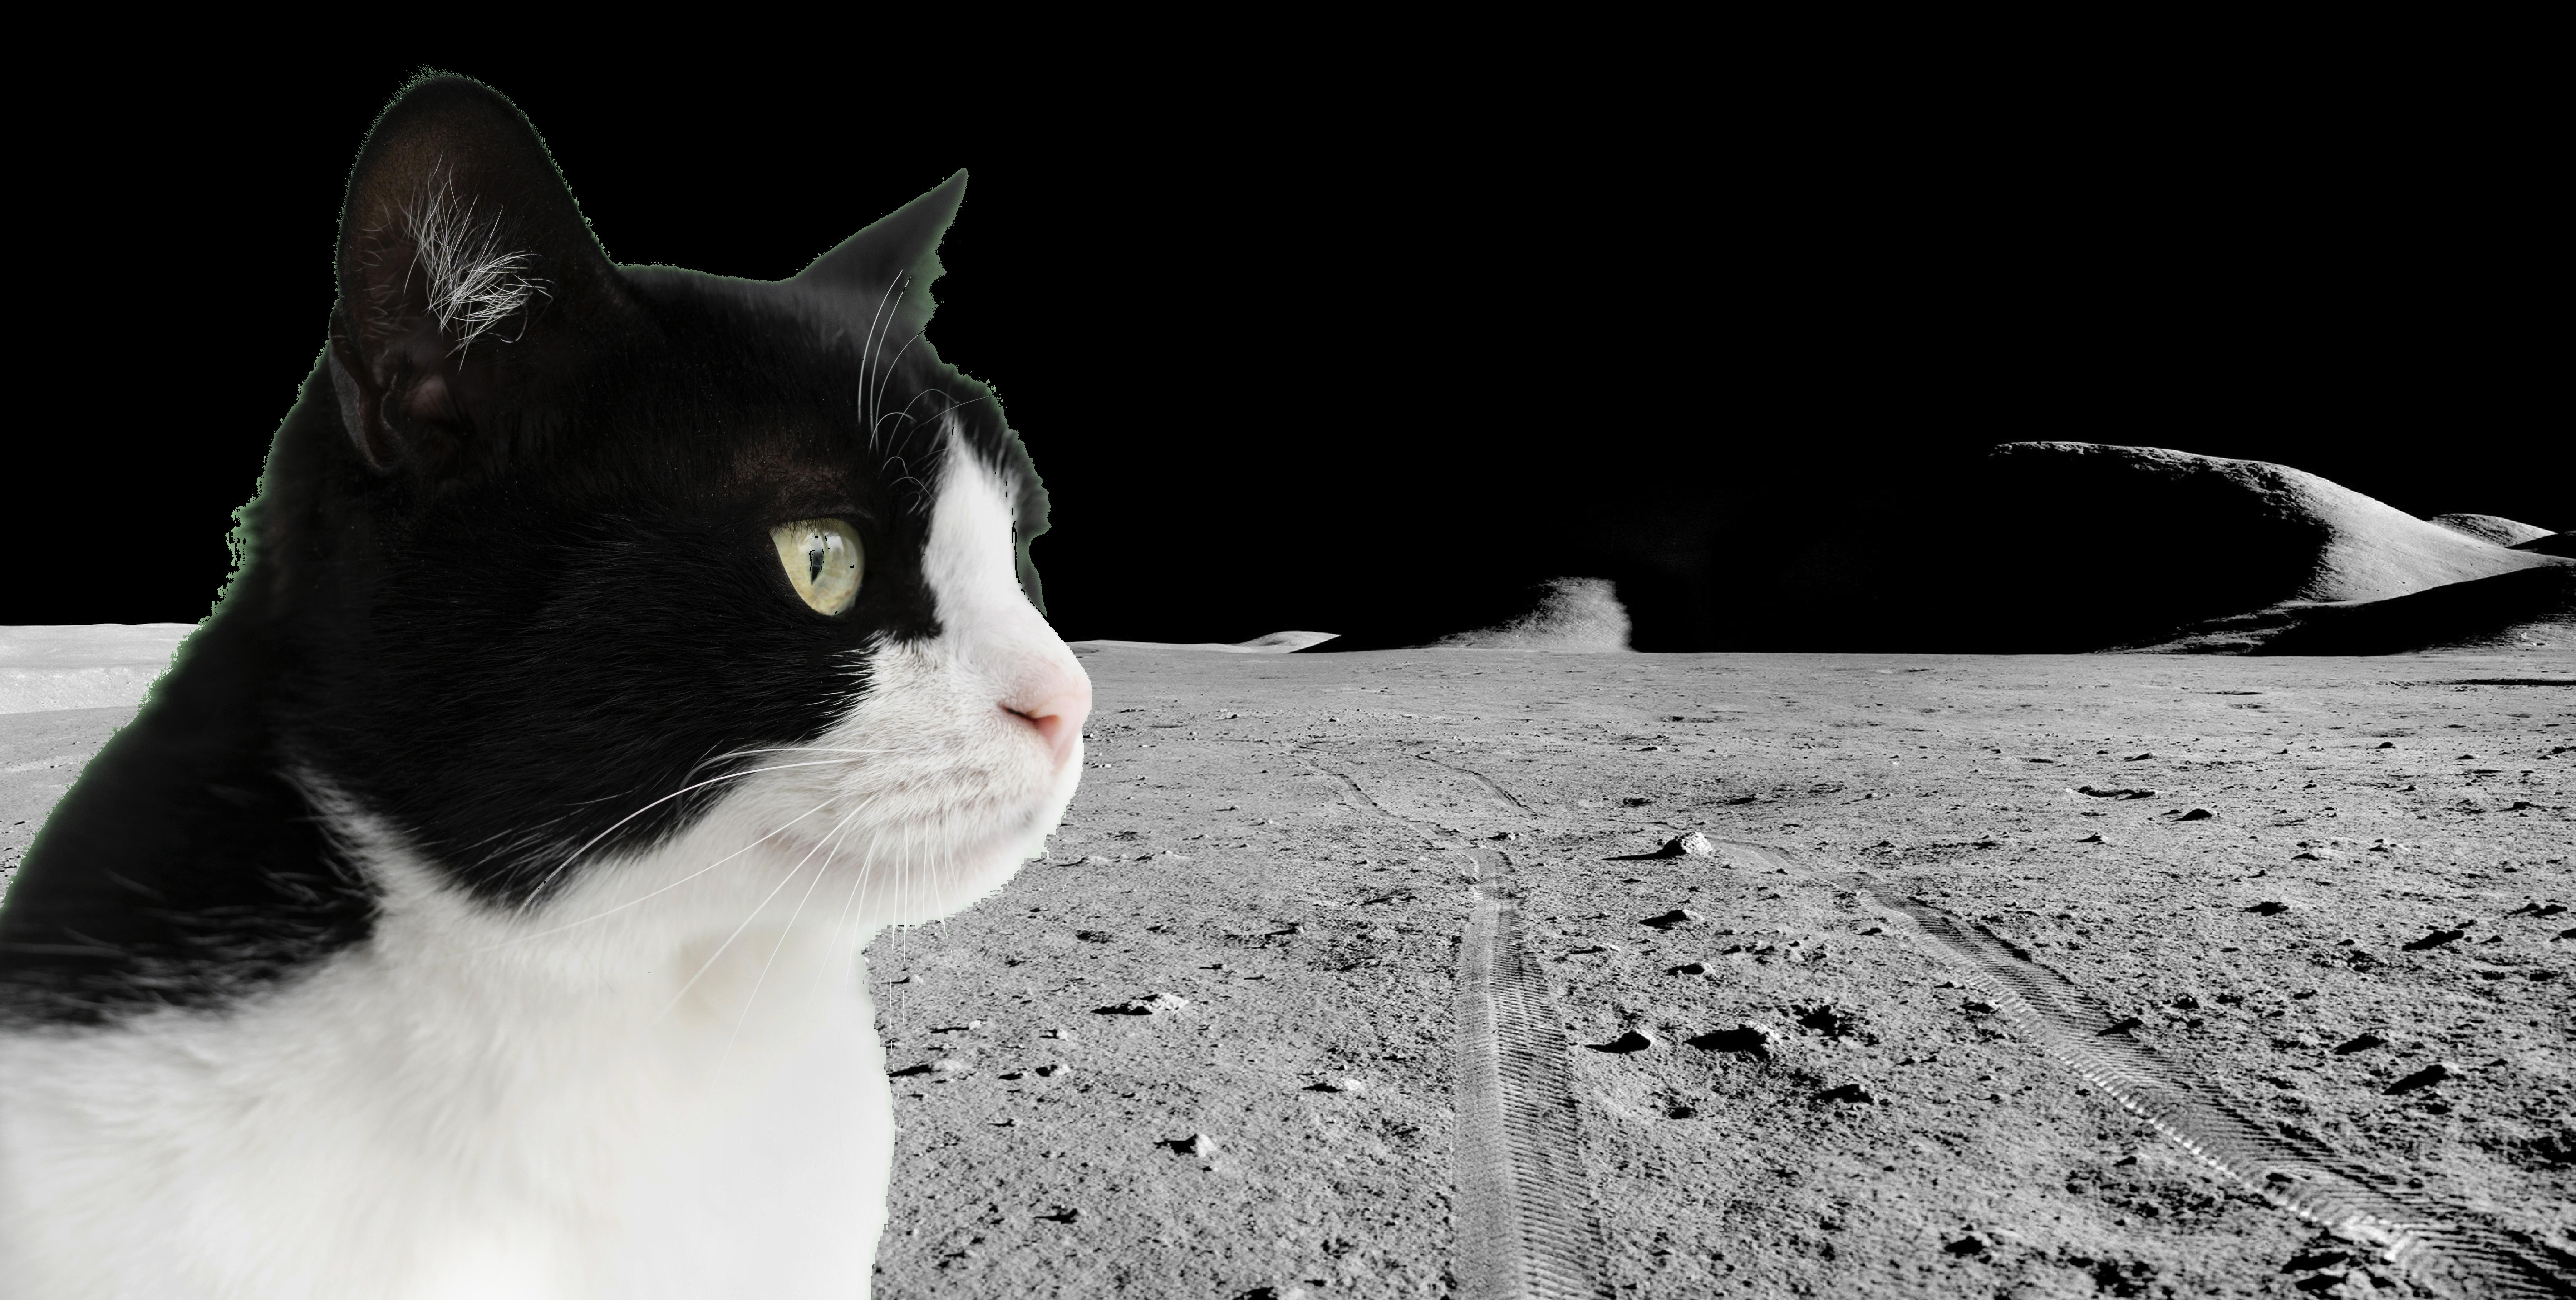
\includegraphics[width=\textwidth]{fig/out/6.comp.jpg}
        \caption{Composited result image.}
    \end{subfigure}

    \caption{Chroma key compositing.}
\end{figure}


\begin{figure}[h!]
    \begin{minted}[ frame=lines, framesep=2mm, linenos ]{matlab} 
im = imread("./media/cat.jpg");
imhsv = rgb2hsv(im);
im_spacebg = imread("./media/spacebg.jpg");

imwrite(im, "./out/6.cat.jpg")
imwrite(im_spacebg, "./out/6.spacebg.jpg")
im = (double(im)./255);
im_spacebg = (double(im_spacebg)./255);

% Lets the user select a pixel in the image to key out.
figure()
imshow(im);
coords = int32(ginput(1));
px_hsv = imhsv(coords(2), coords(1), 1:3);

%  Each channel may deviate of these amounts from the selected pixel.
hue_deviation = 0.05;
saturation_deviation = 0.1; % += 10% saturation
brightness_deviation = 0.4; % += 40% darker/lighter

% Creates the mask for each pixel whose channels are within the deviations
mask = ~((imhsv(:,:,1) > px_hsv(1) - hue_deviation) & (imhsv(:,:,1) < px_hsv(1) + hue_deviation) & ...
        (imhsv(:,:,2) > px_hsv(2) - saturation_deviation) & (imhsv(:,:,2) < px_hsv(2) + saturation_deviation) & ...
        (imhsv(:,:,3) > px_hsv(3) - brightness_deviation) & (imhsv(:,:,3) < px_hsv(3) + brightness_deviation));

im_mask = comp(ones(size(im)),mask,zeros(size(im)));
im_comp = comp(im,mask,im_spacebg);

imshow([im, im_mask, im_comp], []);
title("Original image, mask and composited image")
saveas(gcf,'out/6.image_mask_comp.png')

imwrite(uint8(255.*im_mask), "./out/6.mask.jpg");
imwrite(uint8(255.*im_comp), "./out/6.comp.jpg");


function res = comp(a,mask,b)
    % Masks image 'a' on top of image 'b'
    res = a.*mask + b.*(~mask);
end
    \end{minted}
\caption{Matlab code performing background replacement on image \texttt{cat.jpg}.}
\end{figure}




\subsection{How many bits is enough [2 points]}


\section{Bonus: use your own pictures [3 points]}

\begin{figure}[h!]
    \centering
    \begin{subfigure}{1\textwidth}
        \centering
        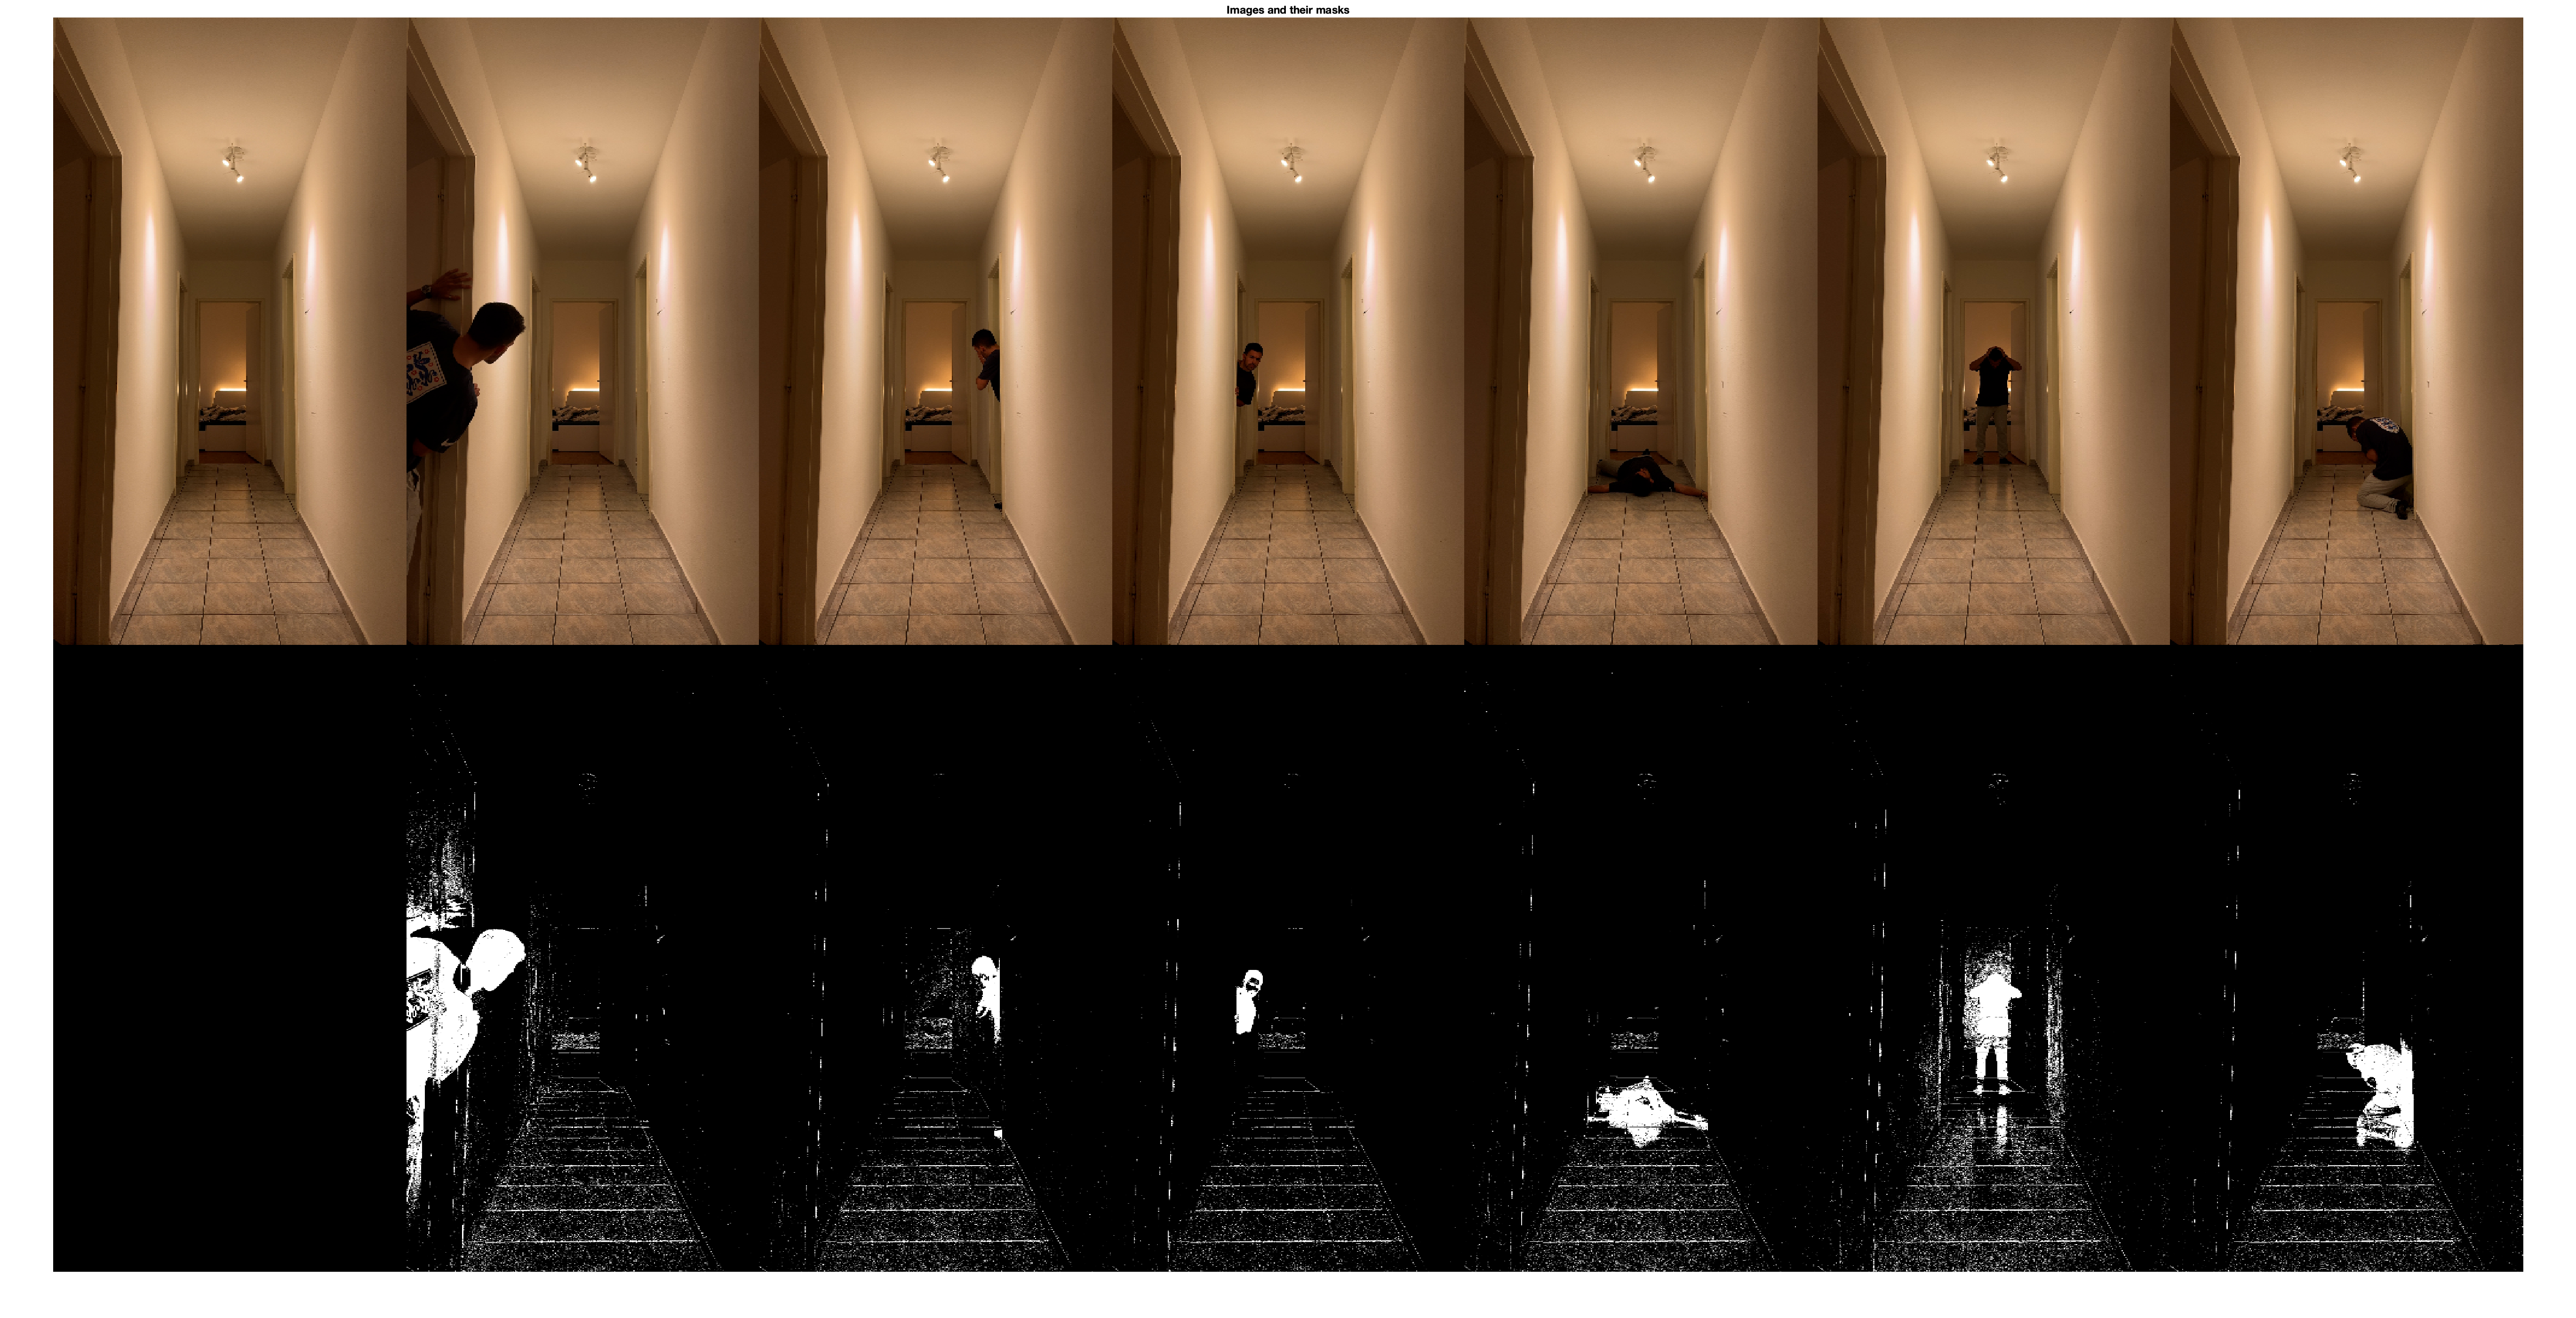
\includegraphics[width=\textwidth]{fig/out/8.images_masks.png}
        \caption{Pictures and relative masks.}
    \end{subfigure}
    
    \begin{subfigure}{0.33\textwidth}
        \centering
        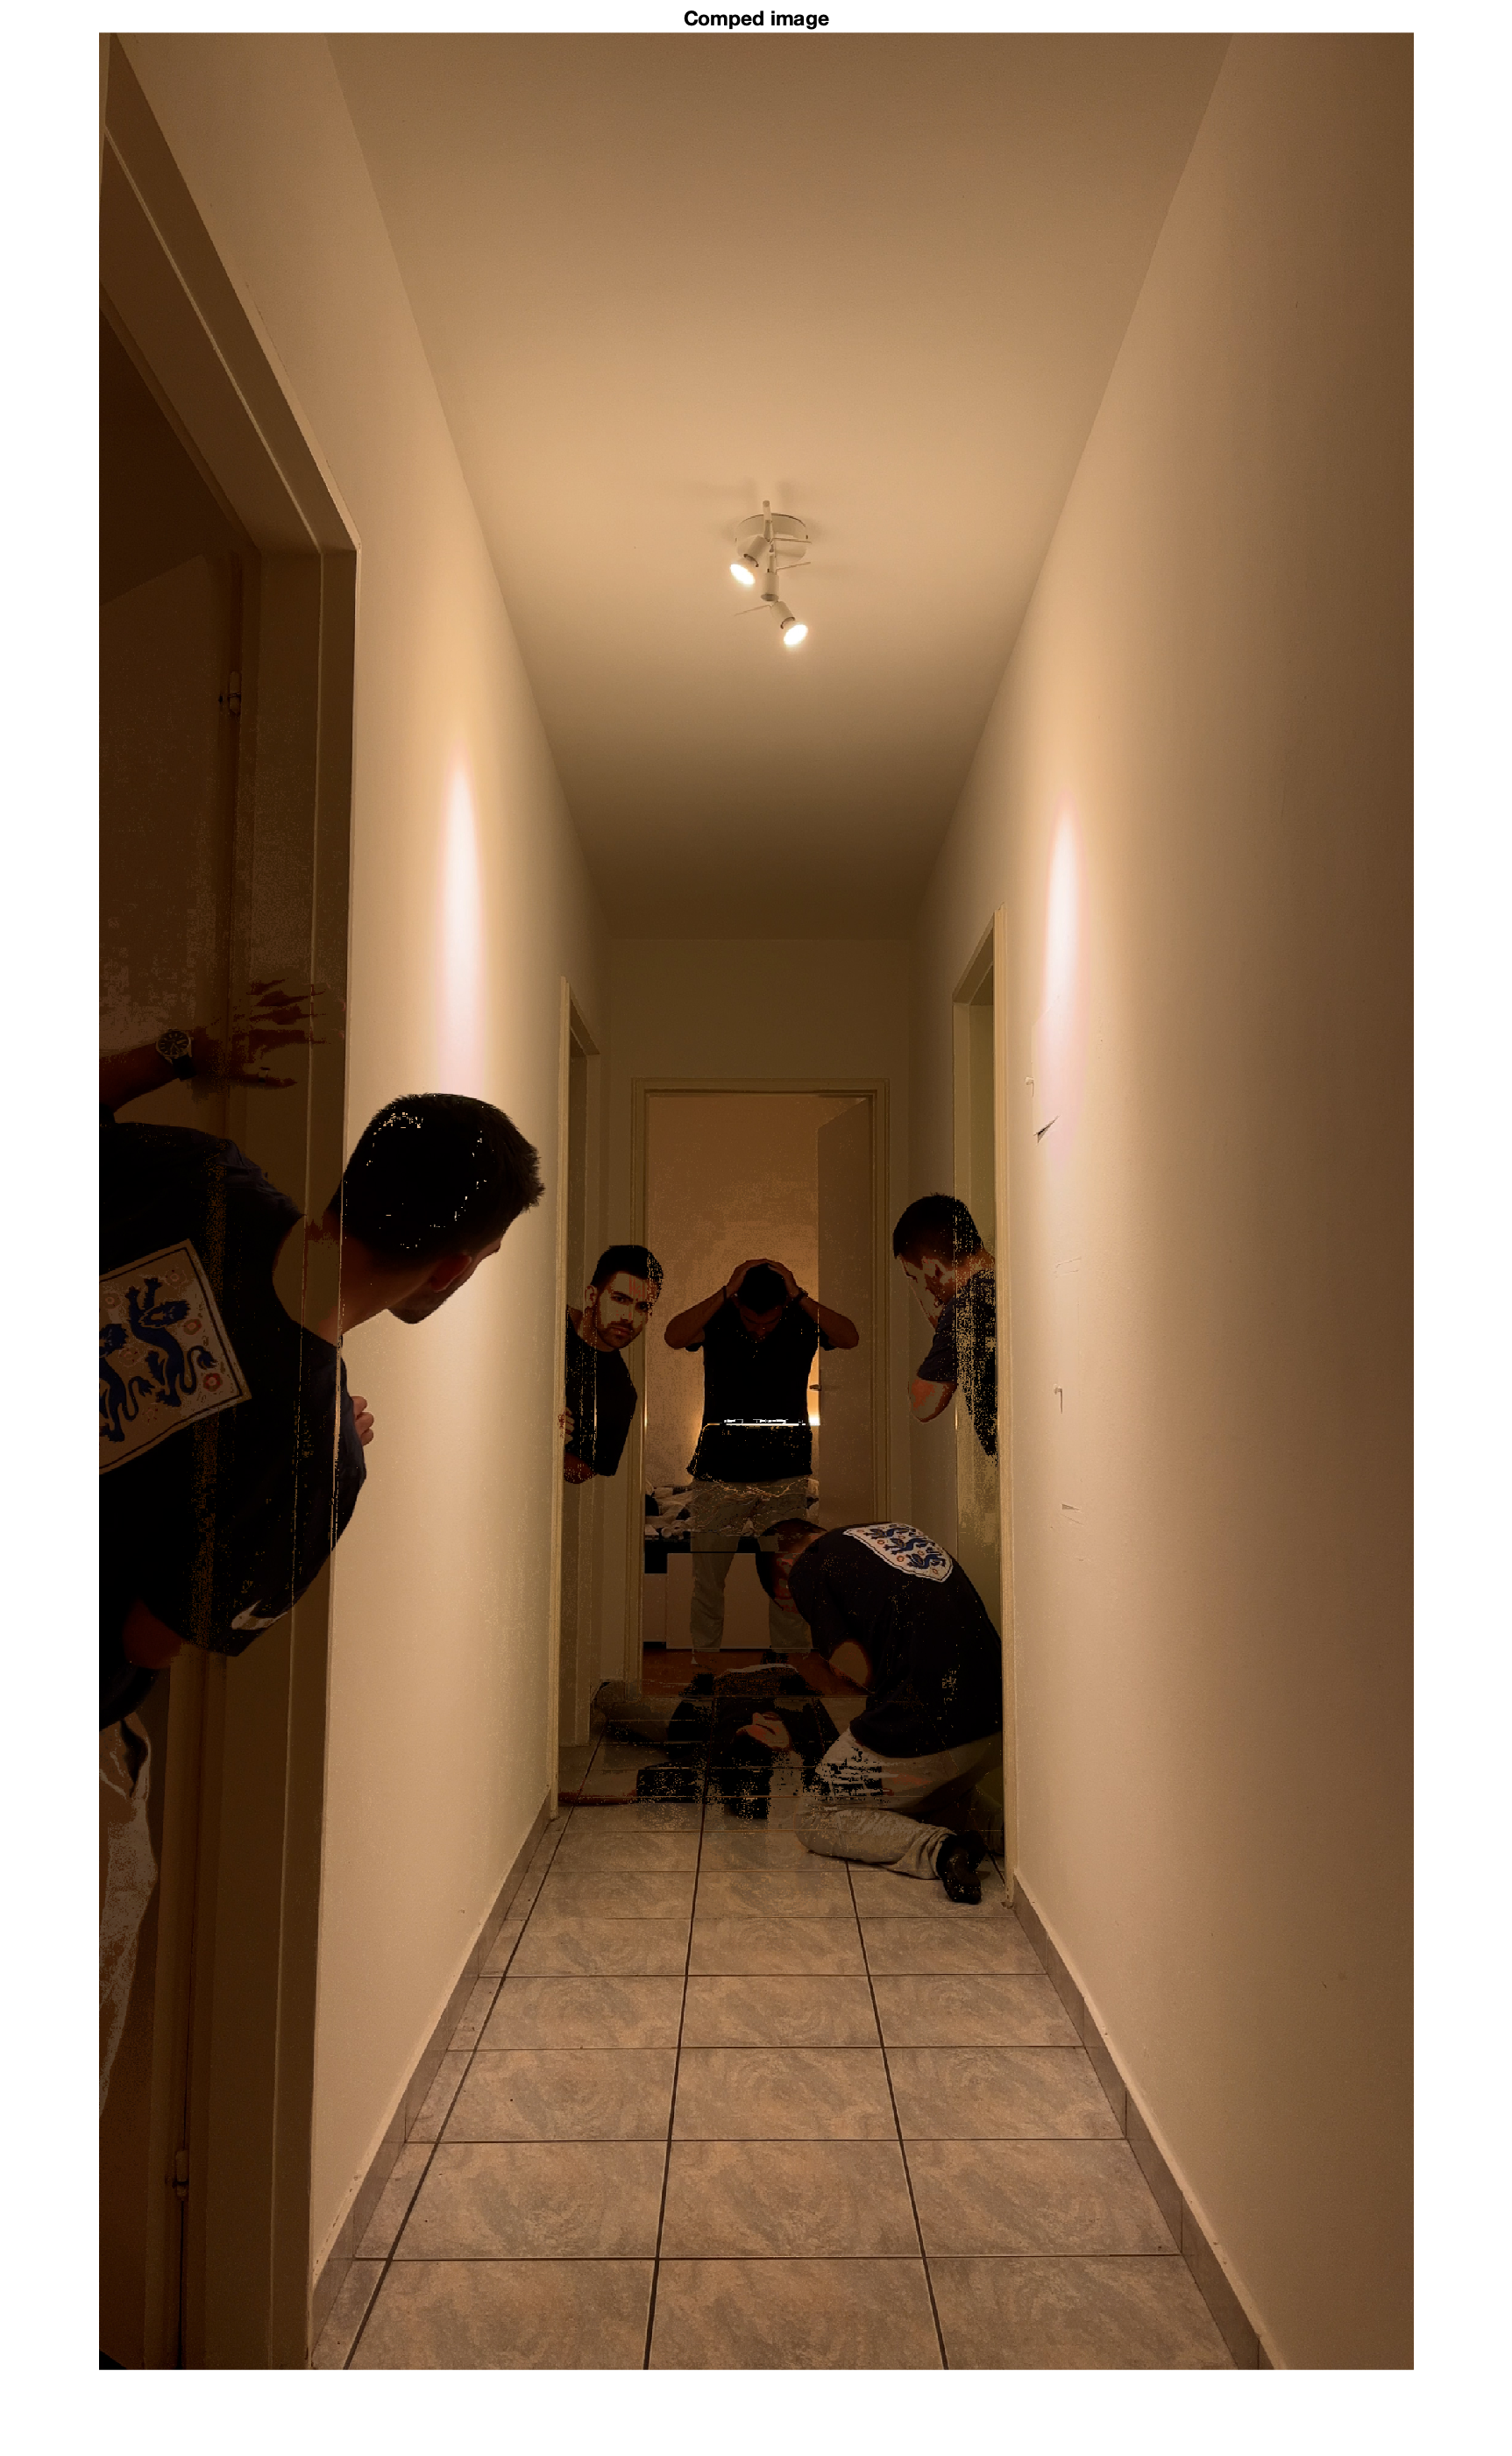
\includegraphics[width=\textwidth]{fig/out/8.im_comped.png}
        \caption{Final composited image}
    \end{subfigure}

    \caption{Compositing myself mutiple times on the same cleanplate.}
\end{figure}


\begin{figure}[h!]
    \begin{minted}[ frame=lines, framesep=2mm, linenos ]{matlab} 
im = imread("./media/cat.jpg");
imhsv = rgb2hsv(im);
im_spacebg = imread("./media/spacebg.jpg");

imwrite(im, "./out/6.cat.jpg")
imwrite(im_spacebg, "./out/6.spacebg.jpg")
im = (double(im)./255);
im_spacebg = (double(im_spacebg)./255);

% Lets the user select a pixel in the image to key out.
figure()
imshow(im);
coords = int32(ginput(1));
px_hsv = imhsv(coords(2), coords(1), 1:3);

%  Each channel may deviate of these amounts from the selected pixel.
hue_deviation = 0.05;
saturation_deviation = 0.1; % += 10% saturation
brightness_deviation = 0.4; % += 40% darker/lighter

% Creates the mask for each pixel whose channels are within the deviations
mask = ~((imhsv(:,:,1) > px_hsv(1) - hue_deviation) & (imhsv(:,:,1) < px_hsv(1) + hue_deviation) & ...
        (imhsv(:,:,2) > px_hsv(2) - saturation_deviation) & (imhsv(:,:,2) < px_hsv(2) + saturation_deviation) & ...
        (imhsv(:,:,3) > px_hsv(3) - brightness_deviation) & (imhsv(:,:,3) < px_hsv(3) + brightness_deviation));

im_mask = comp(ones(size(im)),mask,zeros(size(im)));
im_comp = comp(im,mask,im_spacebg);

imshow([im, im_mask, im_comp], []);
title("Original image, mask and composited image")
saveas(gcf,'out/6.image_mask_comp.png')

imwrite(uint8(255.*im_mask), "./out/6.mask.jpg");
imwrite(uint8(255.*im_comp), "./out/6.comp.jpg");


function res = comp(a,mask,b)
    % Masks image 'a' on top of image 'b'
    res = a.*mask + b.*(~mask);
end
    \end{minted}
\caption{Matlab code performing background replacement on image \texttt{cat.jpg}.}
\end{figure}

\section{Reproducing the results}
In the \verb|src| folder you can find a \verb|Makefile|.
Run \mintinline{shell}{make} to execute the matlab scripts and store the results in the \verb|src/out| folder.\\
Alternatively you can run individual scripts e.g \mintinline{shell}{make src/script1.m}.


\end{document}

